%%%%%%%%%%%%%%%%%%%%%%%%%%%%%%%%%%%%%%%%%
% Sullivan Business Report
% LaTeX Template
% Version 1.0 (May 5, 2022)
%
% This template originates from:
% https://www.LaTeXTemplates.com
%
% Author:
% Vel (vel@latextemplates.com)
%
% License:
% CC BY-NC-SA 4.0 (https://creativecommons.org/licenses/by-nc-sa/4.0/)
%
%%%%%%%%%%%%%%%%%%%%%%%%%%%%%%%%%%%%%%%%%

%----------------------------------------------------------------------------------------
%	CLASS, PACKAGES AND OTHER DOCUMENT CONFIGURATIONS
%----------------------------------------------------------------------------------------

\documentclass[
	a4paper, % Paper size, use either a4paper or letterpaper
	12pt, % Default font size, the template is designed to look good at 12pt so it's best not to change this
	%unnumberedsections, % Uncomment for no section numbering
]{CSSullivanBusinessReport}
\usepackage[T1]{fontenc}
\usepackage[utf8]{inputenc}
%\usepackage{newpxtext}
%\usepackage{newpxmath}
\usepackage{textcomp}
\renewcommand{\ttdefault}{lmtt} % 
%\renewcommand{\ttdefault}{pcr} % pcr is the family name for Courier

%\usepackage{sectsty}
%\usepackage{cite}
\addbibresource{references.bib} % BibLaTeX bibliography file
\addbibresource{sample.bib} % BibLaTeX bibliography file

%----------------------------------------------------------------------------------------
%	REPORT INFORMATION
%----------------------------------------------------------------------------------------

\reporttitle{ARMv8-A72: ARM64 Architecture} % The report title to appear on the title page and page headers, do not create manual new lines here as this will carry over to page headers

\reportsubtitle{Programming for Raspberry Pi 4B\\ \ \\ v\ 1.0} % Report subtitle, include new lines if needed

\reportauthors{Document created by:\\\smallskip \textbf{Ji, Yong-hyeon} (\texttt{hacker3740@kookmin.ac.kr})} % Report authors/group/department, include new lines if needed

\reportdate{\today} % Report date, include new lines for additional information if needed

\rightheadercontent{
\includegraphics[scale=.09]{cse-logo.pdf}} % The content in the right header, you may want to add your own company logo or use your company/department name or leave this command empty for no right header content

%----------------------------------------------------------------------------------------
% PACKAGES
% COLORS
%\usepackage[dvipsnames]{xcolor}  % Include the package with table option
\usepackage{amsthm}

% Define custom theorem styles
\newtheoremstyle{dotless} % Name of the style
{3pt} % Space above
{3pt} % Space below
{\itshape} % Body font
{} % Indent amount
{\bfseries} % Theorem head font
{} % Punctuation after theorem head
{2.5mm} % Space after theorem head
{} % Theorem head spec

\newtheoremstyle{definitionstyle} % Name of the style
{3pt} % Space above
{3pt} % Space below
{} % Body font
{} % Indent amount
{\bfseries} % Theorem head font
{.} % Punctuation after theorem head
{2.5mm} % Space after theorem head
{} % Theorem head spec

% Applying custom styles
%\theoremstyle{dotless}
\newtheorem{theorem}{Theorem} % Theorem environment with section-wise numbering
\newtheorem*{theorem*}{Theorem} % Theorem environment with section-wise numbering
\newtheorem*{corollary*}{Corollary} % Theorem environment with section-wise numbering
\newtheorem{proposition}[theorem]{Proposition} % Theorem environment with section-wise numbering
\newtheorem{lemma}[theorem]{Lemma} % Lemma shares the counter with theorem
\newtheorem{corollary}[theorem]{Corollary} % Corollary shares the counter with theorem

\theoremstyle{definitionstyle}
\newtheorem*{observation}{\textcolor{Magenta}{Observation}}
\newtheorem{terminology}{Terminology} % Example shares the counter with theorem

\newtheorem{definition}{Definition} % Definition shares the counter with theorem
\newtheorem{example}{Example} % Example shares the counter with theorem
\newtheorem{exercise}{{Exercise}} % Example shares the counter with theorem
\newtheorem{remark}{Remark} % Remark shares the counter with theorem
\newtheorem*{note}{Note}

\newtheorem*{terminology*}{Terminology} % Example shares the counter with theorem

\newtheorem*{axiom*}{Axiom}
\newtheorem*{definition*}{Definition} % Definition shares the counter with theorem
\newtheorem*{example*}{Example} % Example shares the counter with theorem
\newtheorem*{exercise*}{\textcolor{violet}{Exercise}} % Example shares the counter with theorem
\newtheorem*{remark*}{Remark} % Remark shares the counter with theorem


\usepackage{tcolorbox}
\tcbset{colback=white, arc=5pt}

\definecolor{axiomcolor}{HTML}{a88bfa}
\definecolor{defcolor}{RGB}{52, 152, 219}
\definecolor{procolor}{RGB}{241, 196, 15}
\definecolor{thmcolor}{RGB}{231, 76, 60}
\definecolor{lemcolor}{RGB}{155, 89, 182}
\definecolor{corcolor}{RGB}{46, 204, 113}
\definecolor{execolor}{RGB}{90, 128, 127}

% Define a new command for the custom tcolorbox
\newcommand{\axiombox}[2][]{%
	\begin{tcolorbox}[colframe=axiomcolor, title={\color{white}\bfseries #1}]
		#2
	\end{tcolorbox}
}

\newcommand{\defbox}[2][]{%
	\begin{tcolorbox}[colframe=defcolor, title={\color{white}\bfseries #1}]
		#2
	\end{tcolorbox}
}

\newcommand{\lembox}[2][]{%
	\begin{tcolorbox}[colframe=lemcolor, title={\color{white}\bfseries #1}]
		#2
	\end{tcolorbox}
}

\newcommand{\probox}[2][]{%
	\begin{tcolorbox}[colframe=procolor, title={\color{white}\bfseries #1}]
		#2
	\end{tcolorbox}
}

\newcommand{\thmbox}[2][]{%
	\begin{tcolorbox}[colframe=thmcolor, title={\color{white}\bfseries #1}]
		#2
	\end{tcolorbox}
}

\newcommand{\corbox}[2][]{%
	\begin{tcolorbox}[colframe=corcolor, title={\color{white}\bfseries #1}]
		#2
	\end{tcolorbox}
}



\usepackage{tikz}
\usepackage{tikz-cd}
\usepackage{tikz-3dplot}
\usepackage{pgfplots}
\usepackage{pgffor} % For \foreach loop
\pgfplotsset{compat=newest} % Adjust to your version of pgfplots
\def\Circlearrowleft{\ensuremath{%
		\rotatebox[origin=c]{180}{$\circlearrowleft$}}}
\def\Circlearrowright{\ensuremath{%
		\rotatebox[origin=c]{180}{$\circlearrowright$}}}
\def\CircleArrowleft{\ensuremath{%
		\reflectbox{\rotatebox[origin=c]{180}{$\circlearrowleft$}}}}
\def\CircleArrowright{\ensuremath{%
		\reflectbox{\rotatebox[origin=c]{180}{$\circlearrowright$}}}}
\usetikzlibrary{
	3d, % For 3D drawing
	angles,
	arrows,
	arrows.meta,
	backgrounds,
	bending,
	calc,
	decorations.pathmorphing,
	decorations.pathreplacing,
	decorations.markings,
	fit,
	matrix,
	patterns,
	patterns.meta,
	positioning,
	quotes,
	shadows,
	shapes,
	shapes.geometric
}
\usepackage{commath}
\usepackage{amsmath, amssymb}   % For math symbols and environments
\usepackage{amsfonts}
\usepackage{graphicx}           % For including images
\usepackage{fancyhdr}           % For headers and footers
\usepackage{hyperref}           % For clickable references
\usepackage{geometry}           % For page margins
\usepackage{color}              % For color text
\usepackage{listings}           % For code listings
\usepackage{caption}            % For customizing figure and table captions
\usepackage{float}              % For floating figures and tables
\usepackage{setspace}


% TABLE
\usepackage{booktabs}
\usepackage[justification=centering]{caption}
\usepackage{tabularx}
\usepackage{multirow}

% LSTLISTING
\usepackage{listings}
\lstdefinestyle{asm}{
	language=[x86masm]Assembler,
	basicstyle=\ttfamily\small,
	keywordstyle=\color{blue},
	commentstyle=\color{gray},
	stringstyle=\color{orange},
	morekeywords={.data, .align, .asciz, .text, .global, .type, .size, .extern, stp, mov, adr, ldr, add, bl, ret, ldp},
	numbers=none
}

% THEOREM
%\theoremstyle{definition}
%\newtheorem{definition}{Definition}[section]
%\newtheorem{theorem}{Theorem}[section]
%\newtheorem{example}{Example}[section]
%----------------------------------------------------------------------------------------

\begin{document}

%----------------------------------------------------------------------------------------
%	TITLE PAGE
%----------------------------------------------------------------------------------------

\thispagestyle{empty} % Suppress headers and footers on this page

\begin{fullwidth} % Use the whole page width
	\vspace*{-0.075\textheight} % Pull logo into the top margin
	
	\hfill
\includegraphics[scale=.15]{cse-logo.pdf} % Company logo

	\vspace{0.15\textheight} % Vertical whitespace

	\parbox{0.9\fulltextwidth}{\fontsize{50pt}{52pt}\selectfont\raggedright\textbf{\reporttitle}\par} % Report title, intentionally at less than full width for nice wrapping. Adjust the width of the \parbox and the font size as needed for your title to look good.
	
	\vspace{0.03\textheight} % Vertical whitespace
	
	{\LARGE\textit{\textbf{\reportsubtitle}}\par} % Subtitle
	
	\vfill % Vertical whitespace
	
	{\Large\reportauthors\par} % Report authors, group or department
	
	\vfill\vfill\vfill % Vertical whitespace
	
	{\large\reportdate\par} % Report date
\end{fullwidth}

\newpage

%----------------------------------------------------------------------------------------
%	DISCLAIMER/COPYRIGHT PAGE
%----------------------------------------------------------------------------------------

\thispagestyle{empty} % Suppress headers and footers on this page

\begin{twothirdswidth} % Content in this environment to be at two-thirds of the whole page width
	\footnotesize % Reduce font size
	
	\subsection*{Disclaimer}

	The information contained in these lecture notes titled "arm64 architecture" is for educational purposes only. The contents are provided "as is" and reflect the author’s views and understanding, developed from academic literature and practical experience. No warranty, express or implied, is made regarding the accuracy, adequacy, completeness, legality, reliability, or usefulness of any information. This disclaimer applies to any errors, omissions, or inaccuracies in the information.
	
	These lecture notes are not endorsed by, directly affiliated with, maintained, authorized, or sponsored by any hardware or software company mentioned. All product and company names are the registered trademarks of their original owners. The use of any trade name or trademark is for identification and educational purposes only and does not imply any association with the trademark holder.
	
	Any use of the information from these notes is at the user’s own risk. In no event shall the author or the Cryptography and Security Engineering Lab be liable for any claims, damages, or other liabilities arising from the use or inability to use the information.

	
	\subsection*{Copyright}
		
	\textcopyright~ 2024 Cryptography and Security Engineering Lab
	All rights reserved.
	
	These lecture notes on arm64 architecture, including all textual content, diagrams, and illustrations, are protected by copyright law and may not be reproduced, distributed, or transmitted in any form or by any means, including photocopying, recording, or other electronic or mechanical methods, without the prior written permission of the author or copyright holder.

	
%	\subsection*{Contact}
	
%	Address Line 1\\
%	Address Line 2\\
%	Address Line 3
	
%	Business Number 123456
	
%	Contact: name@company.com
	
	\vfill % Push the following down to the bottom of the page
	
	\subsubsection*{Changelog}
	
	\scriptsize % Reduce font size further
	
	\begin{tabular}{@{} L{0.05\linewidth} L{0.15\linewidth} L{0.6\linewidth} @{}} % Column widths specified here, change as needed for your content
		\toprule
		v1.0 & 2024-11-08 & Initial release of the arm64 architecture lecture notes, covering all fundamental concepts and basic applications.\\
%		v1.1 & 20XX-02-27 & Pellentesque iaculis odio vel nisl ullamcorper, nec faucibus ipsum molestie.\\
%		v1.2 & 20XX-03-15 & Sed dictum nisl non aliquet porttitor.\\
		\bottomrule
	\end{tabular}
\end{twothirdswidth}

\newpage

%----------------------------------------------------------------------------------------
%	TABLE OF CONTENTS
%----------------------------------------------------------------------------------------

\begin{twothirdswidth} % Content in this environment to be at two-thirds of the whole page width
	\tableofcontents % Output the table of contents, automatically generated from the section commands used in the document
\end{twothirdswidth}

\newpage
%----------------------------------------------------------------------------------------
%	SECTION 1 ARM64 Architecture
%----------------------------------------------------------------------------------------
\section{ARM64 Architecture}

ARM64 (AArch64) is a 64-bit architecture developed by ARM Holdings, widely used in modern mobile devices and servers.\par
ARM64 offers a significant register file structure, with 31 general-purpose registers and special-purpose registers such as the Program Counter (PC) and Stack Pointer (SP). These registers provide flexibility for performing low-level operations efficiently.

\paragraph{Key Features}
\begin{itemize}
	\item 64-bit general-purpose registers (X0-X30).
	\item Special-purpose registers for the stack, program control, and more.
	\item Optimized function calling convention.
\end{itemize}
\subsection{Memory Layout in Computer Systems}

In modern computer systems, memory is divided into several distinct segments that each serve a different purpose in the execution of a program. These segments include the stack, heap, and various regions that hold code and data. This section provides a mathematical description of the layout of memory in a typical system and explains the role of each memory segment.

\subsubsection{Memory Segments}

A typical program is divided into the following memory segments:

\begin{table}[h]
	\centering
	\begin{tabular}{|c|l|}
		\hline
		\multirow{2}{*}{\textbf{Stack}} & Used for local variables, function call management, and control flow. \\
		& It grows downward in memory. \\ \hline
		\multirow{2}{*}{\textbf{Heap}} & Used for dynamic memory allocation (e.g., via \texttt{malloc}). \\ & It grows upward in memory. \\ \hline
		\textbf{.text} & Stores the program's executable instructions (machine code). \\ \hline
		\textbf{.data} & Stores initialized global and static variables. \\ \hline
		\multirow{2}{*}{\textbf{.bss}} & Stores uninitialized global and static variables. \\
		& This segment is initialized to zero at runtime. \\ \hline
		\textbf{.rodata} & Stores read-only data, such as string literals or constant variables. \\ \hline
	\end{tabular}
	%	\caption{Summary of memory segments in a typical program.}
\end{table}
\begin{itemize}
	\item \textbf{Stack:} Used for local variables, function call management, and control flow. It grows downward in memory.
	\item \textbf{Heap:} Used for dynamic memory allocation (e.g., via \texttt{malloc}). It grows upward in memory.
	\item \textbf{.text:} Stores the program's executable instructions (machine code).
	\item \textbf{.data:} Stores initialized global and static variables.
	\item \textbf{.bss:} Stores uninitialized global and static variables. This segment is initialized to zero at runtime.
	\item \textbf{.rodata:} Stores read-only data, such as string literals or constant variables.
\end{itemize}

\noindent The memory layout in a typical process can be visualized as:

\begin{center}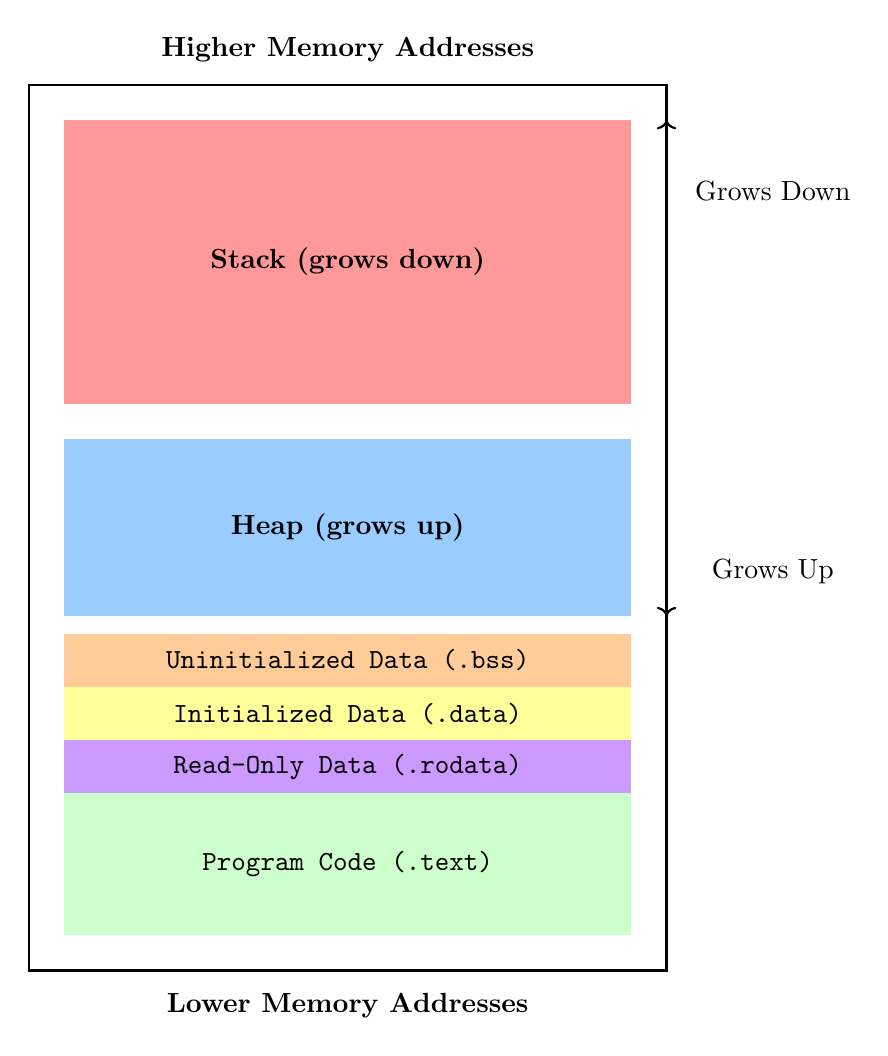
\begin{tikzpicture}[scale=.9]
		% Define colors for segments
		\definecolor{stackcolor}{RGB}{255, 153, 153}
		\definecolor{heapcolor}{RGB}{153, 204, 255}
		\definecolor{textcolor}{RGB}{204, 255, 204}
		\definecolor{datacolor}{RGB}{255, 255, 153}
		\definecolor{bsscolor}{RGB}{255, 204, 153}
		\definecolor{rodatacolor}{RGB}{204, 153, 255}
		
		% Base address
		\node at (0,10.5) {\textbf{Higher Memory Addresses}};
		\node at (0,-3.0) {\textbf{Lower Memory Addresses}};
		
		% Expanded width for rectangles (from -4 to 4)
		% Stack
		\fill[stackcolor] (-4, 5.5) rectangle (4, 9.5);
		\node at (0,7.5) {\textbf{Stack (grows down)}};
		
		% Heap
		\fill[heapcolor] (-4, 2.5) rectangle (4, 5);
		\node at (0,3.75) {\textbf{Heap (grows up)}};
		
		% BSS
		\fill[bsscolor] (-4, 1.5) rectangle (4, 2.25);
		\node at (0,1.875) {\texttt{Uninitialized Data (.bss) }};
		
		% Data
		\fill[datacolor] (-4, 0.75) rectangle (4, 1.5);
		\node at (0,1.125) {\texttt{Initialized Data (.data)}};
		
		% ROData
		\fill[rodatacolor] (-4, 0) rectangle (4, 0.75);
		\node at (0,0.375) {\texttt{Read-Only Data (.rodata)}};
		
		% Text
		\fill[textcolor] (-4, -2) rectangle (4, 0);
		\node at (0,-1) {\texttt{Program Code (.text)}};
		
		% Annotations and arrows
		\draw[thick,->] (4.5,7.5) -- (4.5,9.5);
		\node at (6,8.5) {Grows Down};
		
		\draw[thick,->] (4.5,3.75) -- (4.5,2.5);
		\node at (6,3.125) {Grows Up};
		
		% Memory boundary lines (Expand to match rectangle width)
		\draw[thick] (-4.5, -2.5) rectangle (4.5, 10);
\end{tikzpicture}\end{center}
\newpage
\subsection{Performance Metrics and Benchmarks}
A computer user focuses on minimizing \textbf{response time} (or \textbf{execution time}), while a warehouse-scale operator aims to maximize \textbf{throughput}, the total work completed in a given period.\sidenote{John L. Hennessy and David A. Patterson,
	\textit{Computer Architecture: A Quantitative Approach},
	5th ed., Morgan Kaufmann, 2011.}

We want to relate the performance of two different computers, say, $X$ and $Y$. For the phase \begin{center}
``$X$ is faster than $Y$'',
\end{center} we can define it in terms of execution times: let
\begin{itemize}
	\item \( T_X \) denote the execution time of computer \( X \),
	\item \( T_Y \) denote the execution time of computer \( Y \).
\end{itemize} If \( X \) is faster than \( Y \), then:
\[
T_X < T_Y
\]
This inequality means that the time required for \( X \) to complete the task is less than the time required for \( Y \).

In particular, ``$X$ is $n$ times faster than $Y$''\sidenote{
The computer $X$ is 1.5 times faster than $Y$ means that \[
1.5=\frac{\text{Execution Time}_Y}{\text{Execution Time}_X}.
\] If $\text{Execution Time}_X=10$s and $\text{Execution Time}_Y=15$s, TFAE:
\begin{itemize}
	\item $X$ is 1.5 times faster than $Y$
	\item $Y$ is about 0.76 times slower than $X$.
\end{itemize}
} means that \[
\frac{\text{Execution Time}_Y}{\text{Execution Time}_X}=n.
\] Since execution time is the reciprocal of performance, the following relationship holds:
\[
n = \frac{\text{Execution Time}_Y}{\text{Execution Time}_X} =\frac{\displaystyle 1/\text{Performance}_Y}{\displaystyle 1/\text{Performance}_X}= \frac{\text{Performance}_X}{\text{Performance}_Y}.
\]
where: \begin{itemize}
	\item \( n > 1 \): Computer \( X \) is \( n \) times faster than \( Y \).
	\item \( n < 1 \): Computer \( X \) is \( 1/n\) times slower than \( Y\). In other words, computer $Y$ is $1/n$ times faster than computer $X$.
\end{itemize} 

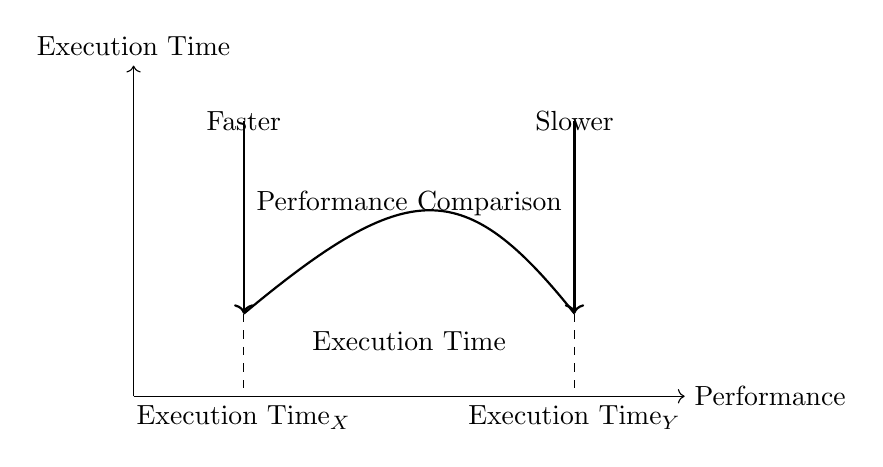
\begin{tikzpicture}[scale=0.7]
	\draw[->] (0,0) -- (10,0) node[right] {Performance};
	\draw[->] (0,0) -- (0,6) node[above] {Execution Time};
	
	\node[align=center] at (2,5) {Faster};
	\node[align=center] at (8,5) {Slower};
	
	\draw[thick, ->] (2,5) -- (2,1.5);
	\draw[thick, ->] (8,5) -- (8,1.5);
	
	% Dotted line for Execution Time X
	\draw[dashed] (2,1.5) -- (2,0) node[below] {$\text{Execution Time}_X$};
	\draw[dashed] (8,1.5) -- (8,0) node[below] {$\text{Execution Time}_Y$};
	
	% Execution Time labels
	\node[align=center] at (5,1) {Execution Time};
	
	% Performance Curve
	\draw[thick] (2,1.5) .. controls (5,4) and (6,4) .. (8,1.5);
	
	% Performance Label
	\node[align=center] at (5,3.5) {Performance Comparison};
\end{tikzpicture}
\newpage
\subsubsection{Quantifying Performance}

Understanding performance is crucial in evaluating computer systems. We use metrics such as \textbf{response time} (or \textit{execution time}) and \textbf{throughput} to measure the efficiency of a system. The relationship between performance and execution time is inversely proportional:
\[
\text{Performance} = \frac{1}{\text{Execution Time}}
\]

This relationship allows us to compare two systems, X and Y:
\[
\text{n} = \frac{\text{Performance}_X}{\text{Performance}_Y} = \frac{\text{Execution Time}_Y}{\text{Execution Time}_X}
\]

\subsubsection{Illustrating Performance Comparison}

The following diagram represents the comparison between two systems, X and Y, in terms of their execution time and throughput:

\begin{center}
	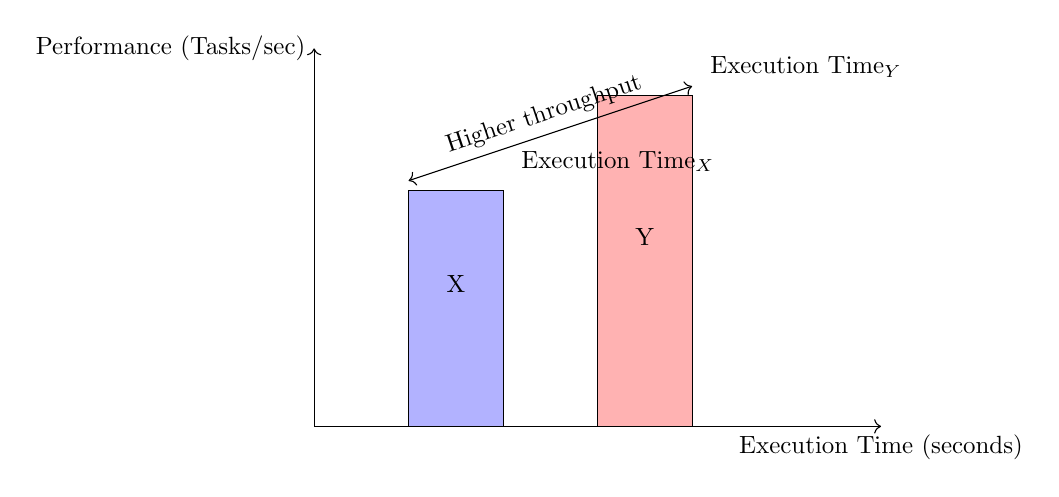
\begin{tikzpicture}[scale=1.2, every node/.style={scale=0.9}]
		% Draw the axes
		\draw[->] (0,0) -- (6,0) node[anchor=north] {Execution Time (seconds)};
		\draw[->] (0,0) -- (0,4) node[anchor=east] {Performance (Tasks/sec)};
		
		% Draw bars for X and Y
		\draw[fill=blue!30] (1,0) rectangle (2,2.5) node[midway, anchor=south, yshift=0.1cm] {X};
		\draw[fill=red!30] (3,0) rectangle (4,3.5) node[midway, anchor=south, yshift=0.1cm] {Y};
		
		% Annotations
		\draw[<->] (1,2.6) -- (4,3.6) node[midway, above, sloped] {Higher throughput};
		\node[anchor=south west] at (2.1, 2.6) {Execution Time$_X$};
		\node[anchor=south west] at (4.1, 3.6) {Execution Time$_Y$};
		
		% Dashed lines for reference
		\draw[dashed] (1,2.5) -- (2,2.5);
		\draw[dashed] (3,3.5) -- (4,3.5);
	\end{tikzpicture}
\end{center}

In this example:
\begin{itemize}
	\item System X has a shorter execution time, indicating higher performance for a given task.
	\item System Y has a longer execution time, leading to lower performance compared to X.
\end{itemize}

\newpage


\newpage

%----------------------------------------------------------------------------------------
%	SECTION 2 GNU Assembly Syntax
%----------------------------------------------------------------------------------------
\section{GNU Assembly Syntax (GAS)}

GNU Assembly (GAS) follows the AT\&T syntax conventions, which differ in operand order and notation from Intel syntax. Below is a structured overview of GAS syntax components and rules.

\newpage

%----------------------------------------------------------------------------------------
%	SECTION 3 Load, Store and Branch Instructions
%----------------------------------------------------------------------------------------
\section{Load, Store and Branch Instructions}

\begin{figure}[h!]
	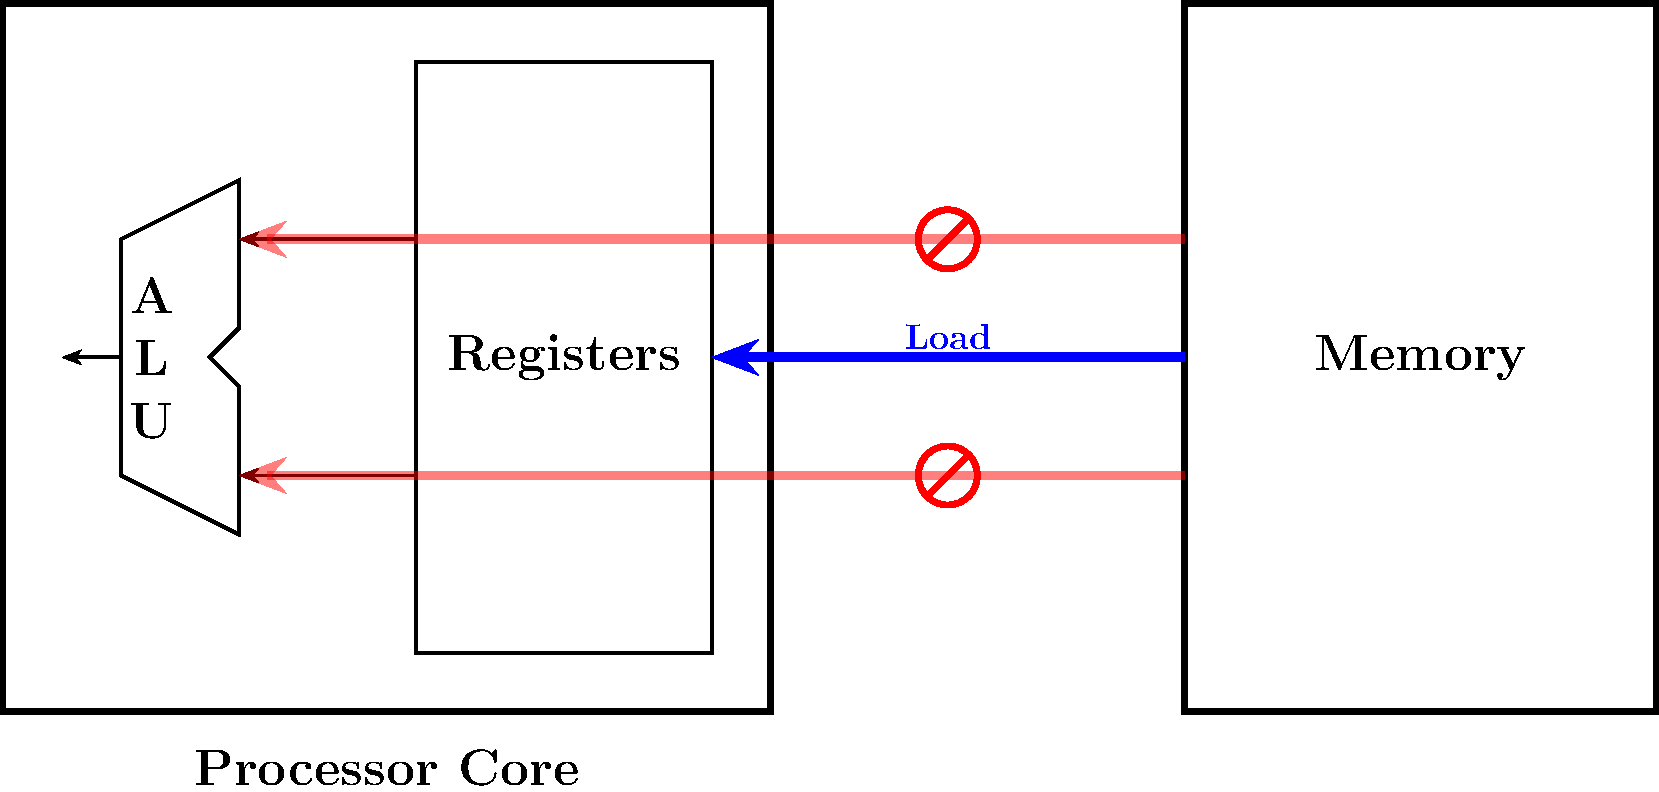
\includegraphics[width=\textwidth]{architectures/load.pdf}
	\caption{Loading Data from Memory}
\end{figure}

\begin{figure}[h!]
	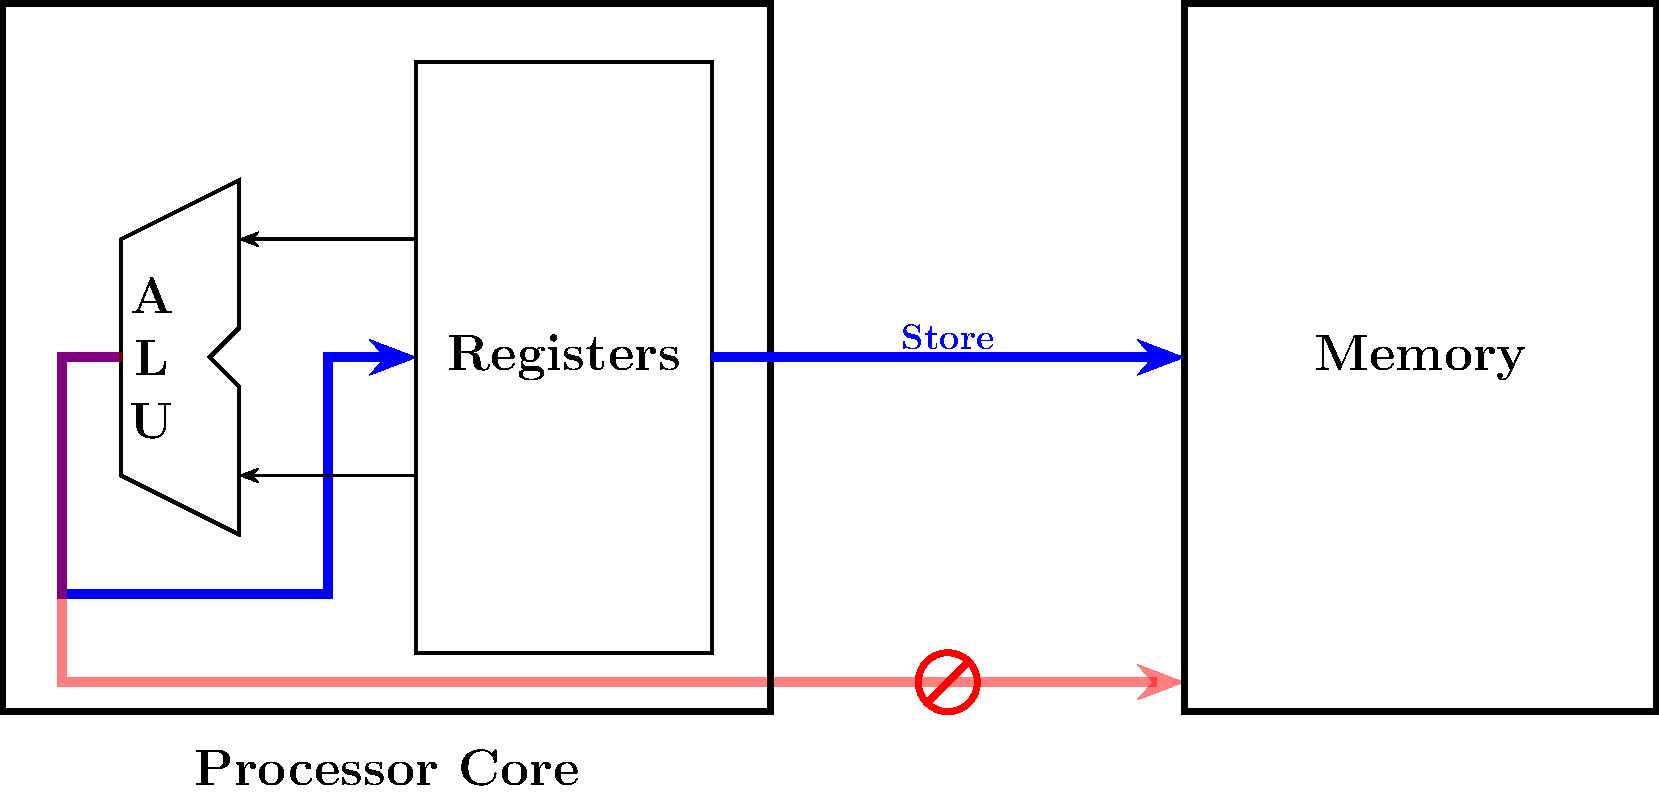
\includegraphics[width=\textwidth]{architectures/store.pdf}
	\caption{Storing Data to Memory}
\end{figure}

\subsection{CPU components and Data paths}
\subsection{AArch64 User Registers}
\begin{itemize}
	\item General purpose registers
	\item Frame pointer
	\item PSTATE register
	\begin{itemize}
		\item Negative
		\item Zero
		\item Carry
		\item oVerflow
	\end{itemize}
	\item Link register
	\item Stack pointer
	\item Zero register
	\item Program counter
\end{itemize}

\subsection{Instruction Components}

\newpage
\subsubsection{Setting and using condition flags}

\begin{example}
\ \begin{table}[h!]\setstretch{1.25}\centering\ttfamily
\caption{Operation Examples}
\begin{tabular*}{\textwidth}{@{\extracolsep{\fill}} c|c||c|c|c|c}
	\toprule[1.2pt]
	\textbf{Operation} & \textbf{Result} & N & Z & C & V \\ \hline
	0x70000000 + 0x70000000 & 0xE0000000 & 1 & 0 & 0 & 1 \\ \hline
	0x80000000 + 0x80000000 & 0x00000000 & 0 & 1 & 1 & 1 \\ \hline
	0x90000000 + 0x90000000 & 0x30000000 & 0 & 0 & 1 & 1 \\ \hline
	0x00001234 - 0x00001000 & 0x00000234 & 0 & 0 & 1 & 0 \\ \hline
	0xFFFFFFFF - 0xFFFFFFFC & 0x00000003 & 0 & 0 & 1 & 0 \\ \hline
	0x80000005 - 0x80000004 & 0x00000001 & 0 & 0 & 1 & 0 \\ \hline
	0x70000000 - 0xF0000000 & 0x80000000 & 1 & 0 & 0 & 1 \\ \hline
	0xA0000000 - 0xA0000000 & 0x00000000 & 0 & 1 & 1 & 0 \\
	\bottomrule[1.2pt]	
\end{tabular*}
\end{table}
\end{example}

Let \begin{align*}
a = a_{31}a_{30}\cdots a_1a_0\in\mathbb{F}_2^{32}\\
b = b_{31}b_{30}\cdots b_1b_0\in\mathbb{F}_2^{32}\\
c = b_{31}c_{30}\cdots c_1c_0\in\mathbb{F}_2^{32},
\end{align*} where $c= a + b\bmod 2^{32}$.
\begin{table}[h!]\setstretch{1.25}\centering
\caption{Flag bits \texttt{NZCV} in \texttt{PSTATE}.}
\begin{tabular*}{\textwidth}{@{\extracolsep{\fill}} c|c|c|c}
	\toprule[1.2pt]
	\multicolumn{2}{c|}{\textbf{Name}} & \textbf{Logical Instruction} & \textbf{Arithmetic Instruction} \\ \cline{0-3}
	\texttt{N} & (Negative) & No meaning & $\texttt{N}=c_{31}$ \\ \cline{0-3}
	\texttt{Z} & (Zero) & Result is all zeroes & $\texttt{Z}=\bigoplus_{i=0}^{31}c_i=0$ \\ \cline{0-3}
	\texttt{C} & (Carry) & - & $\texttt{Z}=\bigoplus_{i=0}^{31}c_i=0$ \\ \cline{0-3}
	\texttt{V} & (oVerflow) & - & $\texttt{Z}=\bigoplus_{i=0}^{31}c_i=0$
\end{tabular*}
\end{table}

\begin{table}[h!]\setstretch{1.25}\centering
\caption{AArch64 condition modifiers.}
\resizebox*{\textwidth}{!}{\begin{tabular}{c|l|c|c}
	\toprule[1.2pt]
	\textbf{Condition Code} & \textbf{Meaning} & \textbf{Condition Flags} & \textbf{Binary Encoding} \\ \hline
	\texttt{EQ} & Equal & $\texttt{Z}=1$ & \texttt{0000} \\
	\texttt{NE} & Not Equal & $\texttt{Z}=0$ & \texttt{0001} \\ \hline
	\texttt{HI} & Unsigned Higher & $(\texttt{C}=1)\land(\texttt{Z}=0)$ & \texttt{1000} \\
\end{tabular}}
\end{table}
\subsubsection{Immediate Values}

\begin{terminology*}
An \textbf{immediate value} in assembly language is a \textit{constant value} that is specified by the programmer.
\end{terminology*}

There are two ways that immediate values can be specified in GNU ARM assembly:
\begin{description}
	\item[(Method 1)] The first way is as a literal immediate value. This can be optionally prefixed with a pound sign for clarity: \begin{center}
		\ttfamily \#<immediate|symbol>
	\end{center}
	\item[(Method 2)] The second way is the \begin{center}
		\ttfamily =<immediate|symbol>
	\end{center} syntax, which can only be used with the `\texttt{ldr}' pseudo-instruction.
\end{description}
\begin{table}[h!]\setstretch{1.25}\centering
\caption{Summary of Valid Immediate Values}
\resizebox*{\textwidth}{!}{\begin{tabular}{c|c|c|c|c}
	\toprule[1.2pt]
	\textbf{Immediate Type} & \textbf{Bits} & \textbf{Description} & \textbf{Legal} & \textbf{Illegal} \\
	Arithmetic & 12 & \\
	Logical & 13 & \\
\end{tabular}}
\end{table}

\newpage
\subsubsection{Addressing Modes}

\begin{table}[h!]\setstretch{1.25}\centering
\caption{Load/Store Memory Addressing Modes}
\resizebox*{1\textwidth}{!}{\begin{tabular}{l|l|l}
	\toprule[1.2pt]
	\textbf{Name} & \textbf{Syntax} & \textbf{Range} \\ \hline
	Register Address & \texttt{[Xn|sp]} & \\
	Singed Immediate Offset & \texttt{[Xn|sp, \#$\pm$<imm9>]} & $\intco{-2^8,2^8}$ \\
	Unsinged Immediate Offset & \texttt{[Xn|sp, \#<imm12>]} & $\intcc{\texttt{0},\texttt{0x7ff8}}$ \\
	Pre-indexed Immediate Offset & \texttt{[Xn|sp, \#$\pm$<imm9>]!} & $\intco{-2^8,2^8}$ \\
	Post-indexed Immediate Offset & \texttt{[Xn|sp], \#$\pm$<imm9>} & $\intco{-2^8,2^8}$ \\
	Register Offset & \texttt{[Xn|sp, Xm, (U|S)XTW]} & (or \texttt{LSL} \#1-3) \\
	Literal & \texttt{label} & $\pm 1$ MB\\
	Pseudo Load & \texttt{=<immediate|symbol>} & 64 bits \\
	\bottomrule[1.2pt]
\end{tabular}}
\end{table}
\vfill\nonumsidenote{\ \\ \ \\
\ttfamily ldr\hspace{1cm} \color{blue}x3\color{black}, \color{red}[x2]\color{gray} \\ \ \\
\color{gray} x3 = memory.word[x2] \\ \ \\
`ldr' stands for Load to Register \\
\ \\ \ \\
\color{black} str\hspace{1cm} \color{blue}x3\color{black}, \color{red}[x2]\color{gray} \\ \ \\
\color{gray} memory.word[x2] = x3 \\ \ \\
`str' stands for Store Register
}
\begin{figure}[h!]
	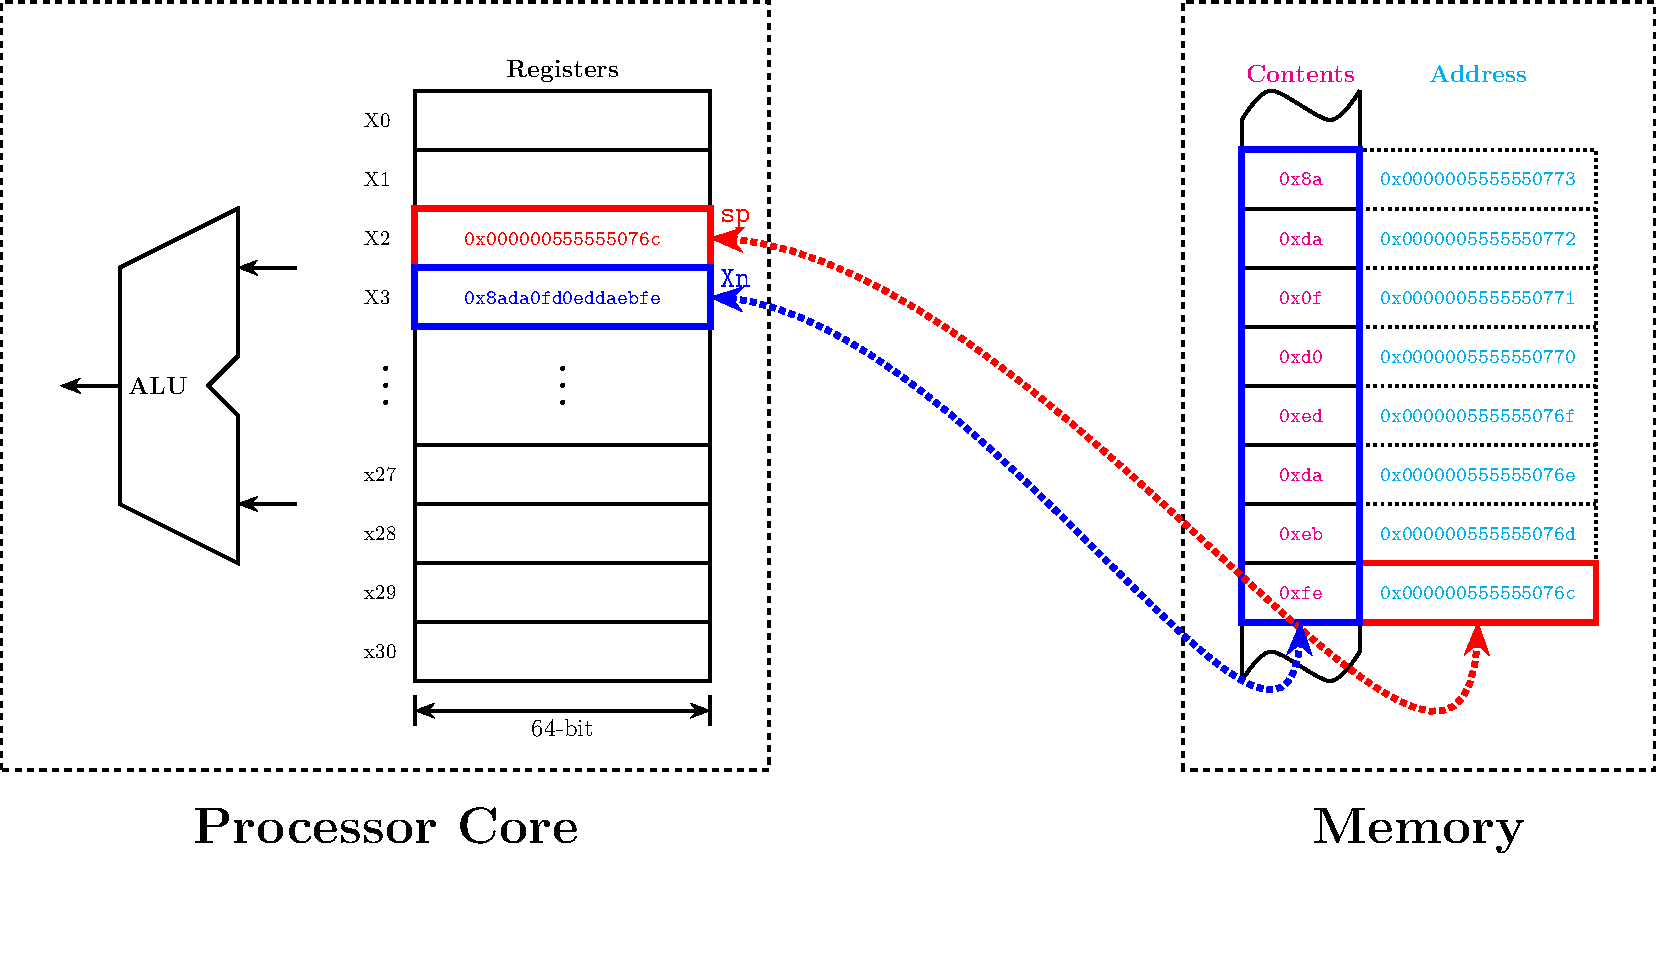
\includegraphics[width=\textwidth]{architectures/register-address.pdf}
	\caption{Access the memory address containing in the
		register \texttt{Xn} or \texttt{sp}.}
\end{figure}
\vfill
\begin{remark*}
	\texttt{[Xn]} or \texttt{[sp]} is just shorthand notation for $\texttt{[Xn,\ \#00]}\ \text{or}\ \texttt{[sp,\ \#00]}$, respectively.
\end{remark*}

\newpage
\nonumsidenote{\ \\ \ \\
	\ttfamily ldur\hspace{.5cm} \color{blue}x0\color{black}, \color{red}[x1, \#0x08] \\ \ \\
	\color{black} stur\hspace{.5cm} \color{blue}x0\color{black}, \color{red}[x1, \#-0x08]\color{gray} 
}
\begin{figure}[h!]
	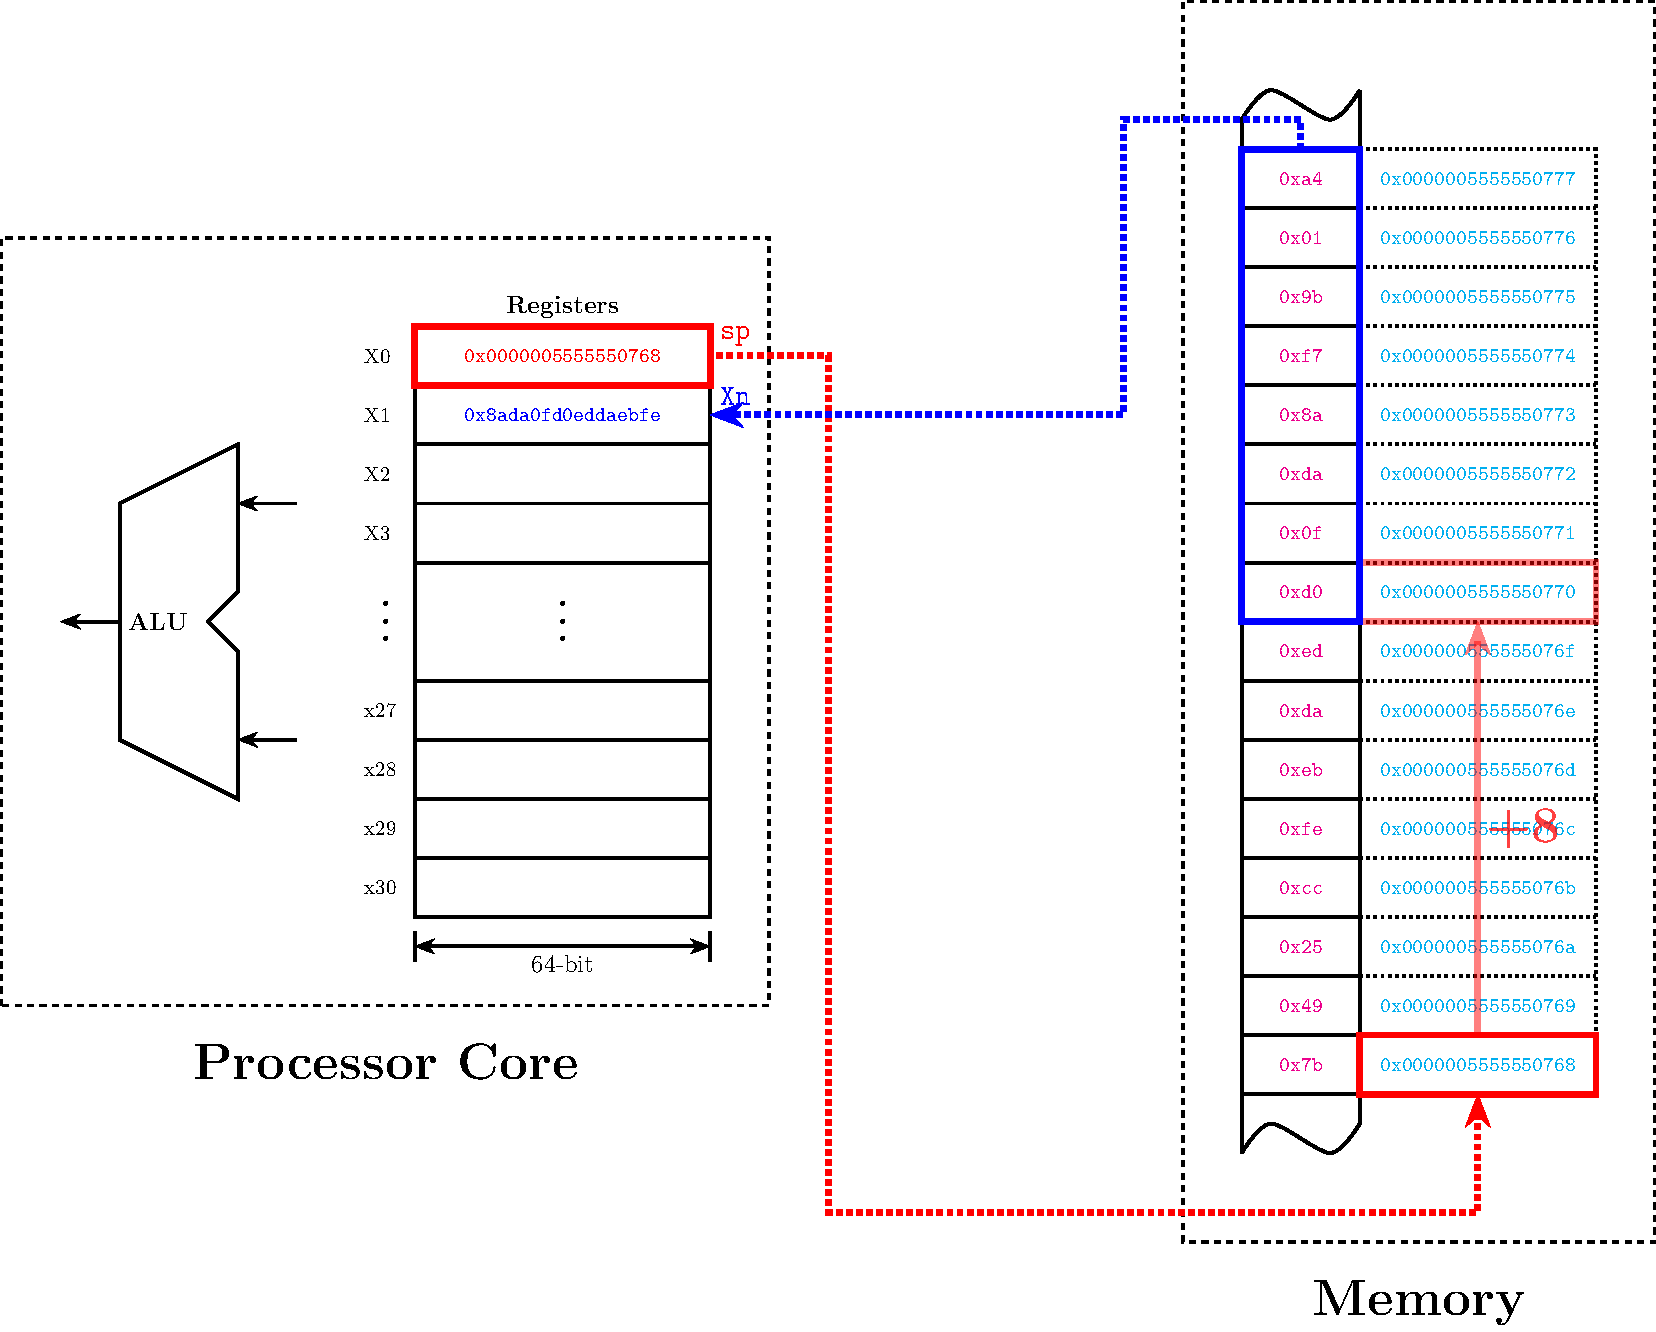
\includegraphics[width=\textwidth]{architectures/immediate-offset.pdf}
	\caption{Signed Immediate Offset.}
\end{figure}

\begin{table}[h!]\setstretch{1.25}\centering
\caption{Pre-index, Post-index and Pre-index with Update}
\resizebox*{1\textwidth}{!}{\begin{tabular}{l|l}
	\toprule[1.2pt]
	\multirow{3}{*}{\textbf{Pre-index}} & \texttt{ldr\hspace{1cm} X1,\ [X0, \#0x08]} \\ \cline{2-2}
	& \texttt{X1 $\gets$ memory.word[X0 + 0x08]} \\
	& \texttt{X0} remains unchanged \\ \hline
	\multirow{3}{*}{\textbf{Post-index}} & \texttt{ldr\hspace{1cm} X1,\ [X0],\ \#0x08} \\ \cline{2-2}
	& \texttt{X1 $\gets$ memory.word[X0]} \\
	& \texttt{X0 $\gets$ X0 + 0x08} \\ \hline
	\multirow{3}{*}{\textbf{Pre-index with Update}} & \texttt{ldr\hspace{1cm} X1,\ [X0, \#0x08]!} \\ \cline{2-2}
	& \texttt{X1 $\gets$ memory.word[X0 + 0x08]} \\
	& \texttt{X0$\gets$ X0 + 0x08}\\
	\bottomrule[1.2pt]
\end{tabular}}
\end{table}

\newpage
\subsection{Load and Store Instructions}
The load and store instructions allow the programmer to move data from memory to registers
or from registers to memory. The load/store instructions can be grouped into the following
types:
\begin{itemize}
	\item single register,
	\item register pair,
	\item atomic.
\end{itemize}

\subsubsection{Load/store single register}
These instructions transfer a double-word(64-bit), single word(32-bit), half-word(16-bit), or byte(8-bit) from a register to memory or from memory to a register:

\begin{table}[h!]
\begin{tabular}{ll}
	\texttt{\bf ldr} & Load Register \\
	\texttt{\bf str} & Store Register
\end{tabular}
\end{table}

\begin{figure}[h!]\centering
	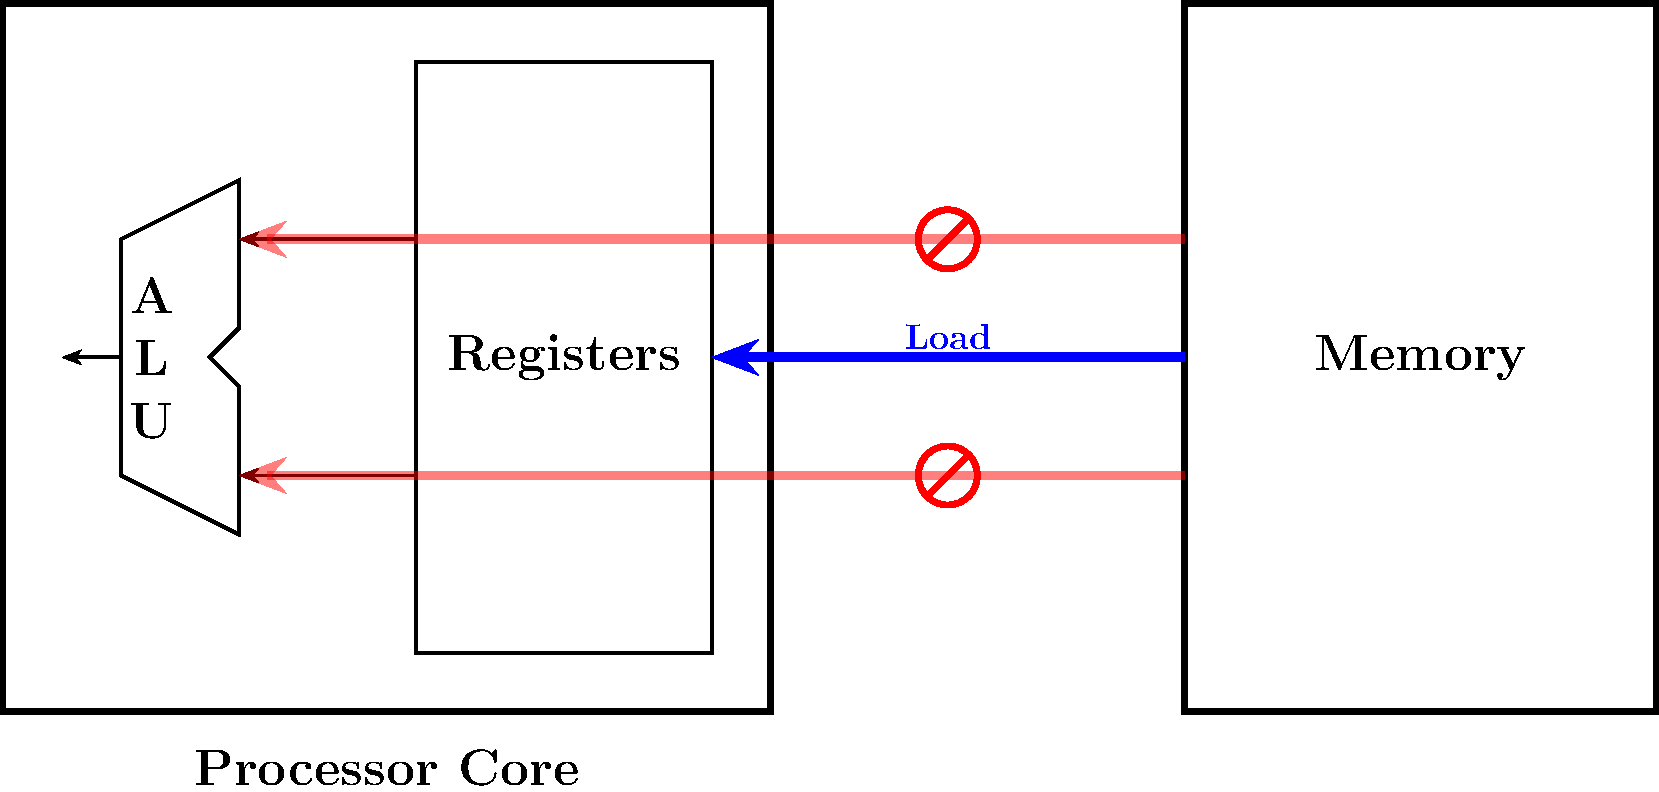
\includegraphics[width=.975\textwidth]{architectures/load.pdf}
	\caption{Loading Data from Memory}
\end{figure}

\begin{figure}[h!]\centering
	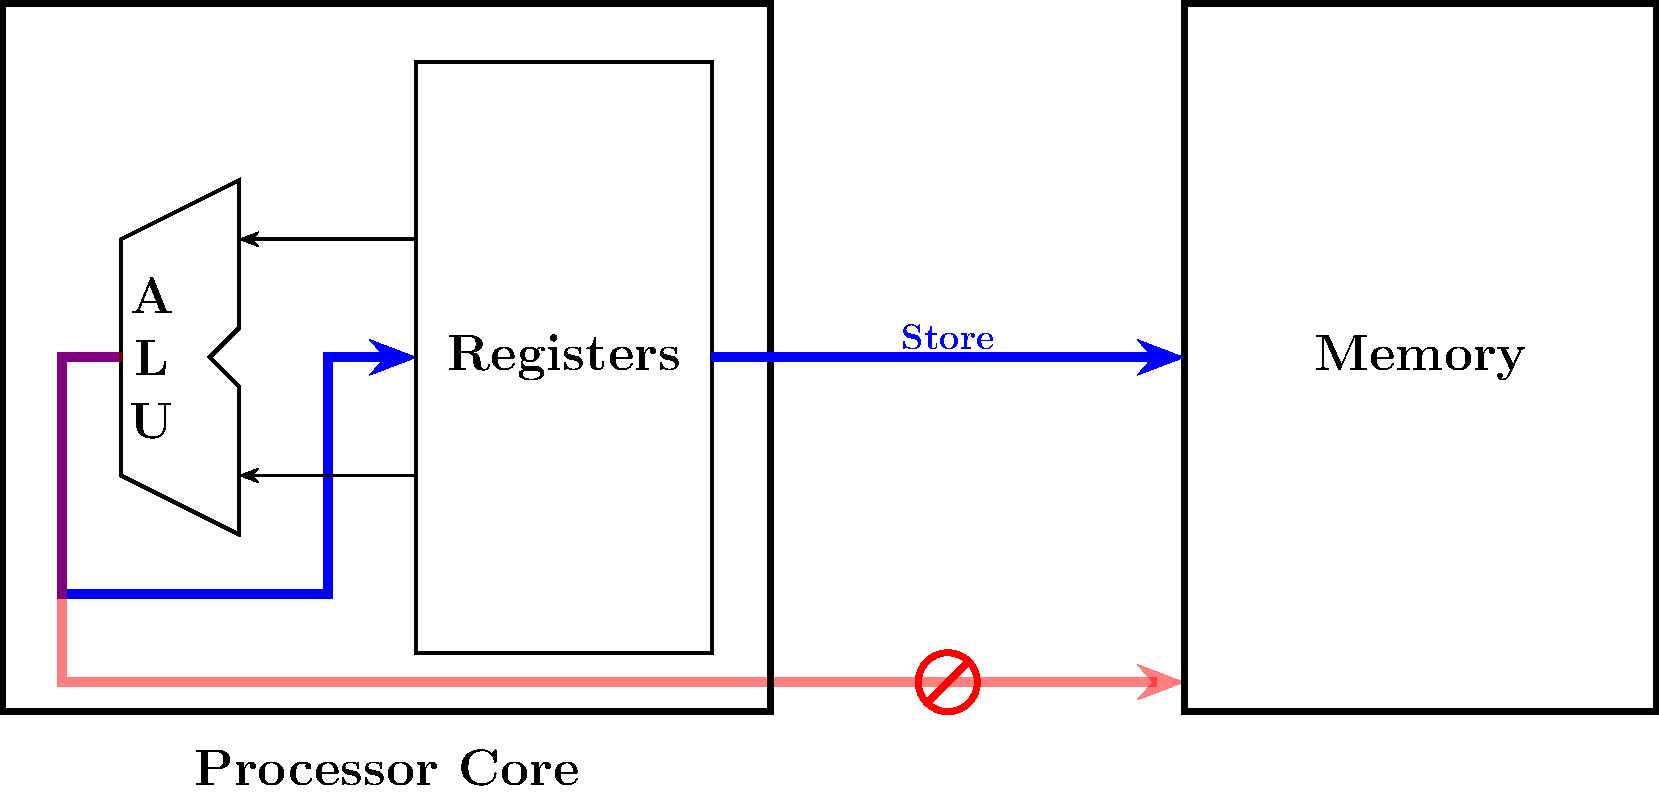
\includegraphics[width=.975\textwidth]{architectures/store.pdf}
	\caption{Storing Data to Memory}
\end{figure}

\newpage
\begin{description}
	\item[Syntax] \boxed{\texttt{<op>\{<size>\}\hspace{.5cm} Rd, <addr>}}
	\nonumsidenote{\begin{itemize}[leftmargin=*]
			\item \texttt{<op>} is either \texttt{ldr} or \texttt{str}.
			\item The optional \texttt{<size>} is one of: \begin{center}
			\ttfamily b,\quad h,\quad sb,\quad sh,\quad sw
			\end{center}
			\item[] \texttt{b}: unsigned byte
			\item[] \texttt{h}: unsigned half-word
			\item[] \texttt{sb}: signed byte
			\item[] \texttt{sh}: signed half-word
			\item[] \texttt{sw}: signed word
			\item \texttt{str} cannot use a singed \texttt{<size>}. It also cannot use the literal addressing mode.
	\end{itemize}}
	\item[Operation] \ \begin{table}[h!]
		\begin{tabular}{lll}
			\textbf{Name} & \textbf{Effect} & \textbf{Description} \\ \hline
			\texttt{ldr} & \texttt{Rd $\gets$ Mem[addr]} & Load register from memory at \texttt{addr} \\ \hline
			\texttt{str} & \texttt{Mem[addr] $\gets$ Rd} & Store register in memory at \texttt{addr}
		\end{tabular}
	\end{table}
\end{description}

\begin{example*} \ \\ 
\begin{lstlisting}
	// Load the word (4 byte) value
	// from Mem[x4] into w8,
	// and set the upper four bytes of x8to zero.
	ldr		w8, [x4]
\end{lstlisting}
\begin{figure}[h!]\centering
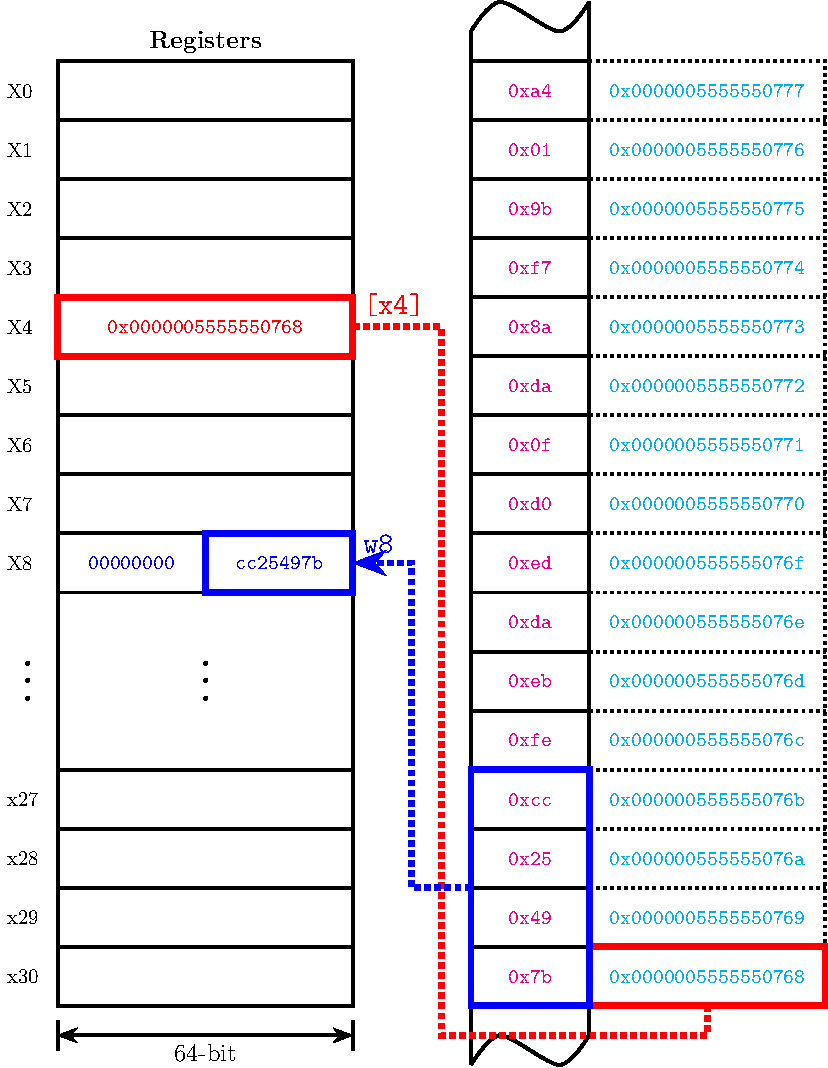
\includegraphics[width=.9\textwidth]{architectures/load-store-example1.pdf}
\caption{Load the word (4 byte) value from \texttt{Mem[x4]} into \texttt{w8}, and set the upper four bytes of \texttt{x8} to zero.}	
\end{figure}
\newpage
\begin{lstlisting}
	// Store the least-significant byte
	// from register x12 into Mem[x2].
	strb		x12, [x2]
\end{lstlisting}
\begin{lstlisting}
	// Load the double-word (8 byte) value
	// from Mem[x3 + 7] into x5. Then set x3 = x3 + 7:
	ldr		x5, [x3, #7]!
\end{lstlisting}
\begin{lstlisting}
	// Store the half-word (2 byte) value
	// in w9 to Mem[x6]. Then set x6 = x6 + 7:
	strh		w9, [x6], #7
\end{lstlisting}
\begin{lstlisting}
	// Load the half-word value
	// from Mem[x0 + 8] into x5 and sign extend it:
	ldrsh		x5, [x0, 8]
\end{lstlisting}
\begin{lstlisting}
	// Store the least significant byte
	// in w1 at Mem[x9]:
	strb		w1, [x9]
\end{lstlisting}
\end{example*}

\subsubsection{Load/store single register (unscaled)}
These instructions are the same as Load/Store Single Register, except that they only use an
unscaled, signed addressing mode with an offset range of $\intcc{-256,256}$. \nonumsidenote{Programmers rarely need to write \texttt{ldur} or \texttt{stur} explicitly. The programmer can just use \texttt{ldr} or \texttt{str}, and the assembler will almost always automatically convert them to \texttt{ldur} or \texttt{stur} when appropriate.}
\begin{table}[h!]
	\begin{tabular}{ll}
		\texttt{\bf ldur} & Load Register (Unscaled) \\
		\texttt{\bf stur} & Store Register (Unscaled)
	\end{tabular}
\end{table}
\begin{description}
\item[Syntax] \boxed{\texttt{<op>\{<size>\}\hspace{.5cm} Rd, [Xn, \#imm9]}}
\item[Operation] \ \begin{table}[h!]
	\begin{tabular}{lll}
		\textbf{Name} & \textbf{Effect} & \textbf{Description} \\ \hline
		\texttt{ldur} & \texttt{Rd $\gets$ Mem[addr]} & Load register from memory at \texttt{addr} \\ \hline
		\texttt{stur} & \texttt{Mem[addr] $\gets$ Rd} & Store register in memory at \texttt{addr}
	\end{tabular}
\end{table}
\end{description}
\begin{example*}
\ \begin{lstlisting}
	// Load the byte value from Mem[x5 + 255]. 
	// Sign extend it and store the value in x4:
	ldursb		x4, [x5, #255]
\end{lstlisting}
\begin{lstlisting}
	// Store the double-word value in x1 to Mem[x2 - 256]:
	stur		x1, [x2, #-256]
\end{lstlisting}
\end{example*}

\subsubsection{Load/store pair}
These instructions are used to store or load two registers at a time. This can be useful for moving registers onto the stack or for copying data. These two instructions are particularly useful for transferring data in a load-store architecture because each instruction can move twice as much information as the \texttt{ldr} and \texttt{str} instructions.

\begin{table}[h!]
	\begin{tabular}{ll}
		\texttt{\bf ldp} & Load Pair \\
		\texttt{\bf stp} & Store Pair
	\end{tabular}
\end{table}
\begin{description}
	\item[Syntax] \boxed{\texttt{<op>\{<size>\}\hspace{.5cm} Rt, Rt2, <addr>}}
	\nonumsidenote{\begin{itemize}[leftmargin=*]
			\item \texttt{<op>} is either \texttt{ldp} or \texttt{stp}.
			\item The optional \texttt{<size>} is optionally \texttt{sw} for signed words.
			\item \texttt{<addr>} is 7 bits Pre-indexed, Post-indexed, or Signed immediate.
			\item Signed immediate
			\item[] \texttt{Xt} range: $[\texttt{-0x200, 0x1f8}]$.
			\item[] \texttt{Wt} range: $[\texttt{-0x100, 0xfc}]$.
	\end{itemize}}
	\item[Operation] \ \begin{table}[h!]
		\begin{tabular}{lll}
			\textbf{Name} & \textbf{Effect} & \textbf{Description} \\ \hline
			\multirow{5}{*}{\texttt{ldp}} & & Load register pair\\
			& \texttt{Rt $\gets$ Mem[addr]}&  from memory at \texttt{addr}\\
			& \texttt{Rt2 $\gets$ Mem[addr + size(Rt)]} & where \texttt{sizeof(Rt)} is \\
			& & 4 for \texttt{Wt} registers \\
			& & and 8 for \texttt{Xt} registers \\ \hline
			\multirow{2}{*}{\texttt{stur}} & \texttt{Mem[addr] $\gets$ Rd} & Store register pair \\
			& \texttt{Mem[addr + size(Rt)] $\gets$ Rt2} & in memory at \texttt{addr}
		\end{tabular}
	\end{table}
\end{description}
\begin{example*}
	\ \begin{lstlisting}
		// Load the byte value from Mem[x5 + 255]. 
		// Sign extend it and store the value in x4:
		ldursb		x4, [x5, #255]
	\end{lstlisting}
	\begin{lstlisting}
		// Store the double-word value in x1 to Mem[x2 - 256]:
		stur		x1, [x2, #-256]
	\end{lstlisting}
\end{example*}

\subsubsection{Summary}

\newpage
\subsection{Branch instructions}
Branch instructions allow the programmer to change the address of the next instruction to be
executed. They are used to implement loops, if-then structures, subroutines, and other flow
control structures. There are five instructions related to branching:
\begin{itemize}
	\item Branch,
	\item Branch to Register,
	\item Branch and Link (subroutine call),
	\item Compare and Branch, and
	\item Form program-counter-relative Address.
\end{itemize}

\subsubsection{Branch}
\newpage

%----------------------------------------------------------------------------------------
%	SECTION 4 Data Processing and Other Instructions
%----------------------------------------------------------------------------------------
\section{Data Processing and Other Instructions}

\subsection{Arithmetic Operations}
\nonumsidenote{There are six basic arithmetic operations:
\begin{tabular}{ll}
	\texttt{add} & Addition \\
	\texttt{adc} & Addition with Carry \\
	\texttt{sub} & Subtract \\
	\texttt{suc} & Subtraction with Carry \\
	\texttt{neg} & Negate \\
	\texttt{ngc} & Negate with Carry \\
\end{tabular}}
\begin{lstlisting}
#include <stdio.h>
static int x = 5;
static int y = 8;
int main(void) {
	int sum;
	sum = x + y;
	printf("The sum is %d\n",sum);
	return 0;
}
\end{lstlisting}
\nonumsidenote{\begin{itemize}[leftmargin=*]
	\item \textbf{Data Segment}:
	\item[*] \texttt{fmt} holds \texttt{"The sum is \%d\textbackslash n\textbackslash0"}.
	\item[*] \texttt{x} contains the integer \texttt{5}.
	\item[*] \texttt{y} contains the integer \texttt{8}.
	\item \textbf{Stack Frame during main Execution}:
	\item[*] Temporary space for \texttt{x29} and \texttt{x30}.
	\item[*] Stack pointer adjusts as needed for the function call and return.
\end{itemize}}
\begin{lstlisting}
		.data
fmt:	.asciz	"The sum is %d\n"
		.algin	2
x:		.word 	5
y:		.word 	8
		.text
		.type 	main, %function
		.global	main
main:
		stp 	x29, x30, [sp, #-16]! 	// Push FP, LR onto the stack
		//	sum = x + y
		adr 	x14, x					// Calculate address of x
		adr 	x15, y					// Calculate address of y 
		ldr 	x4, [x14] 				// Load x
		ldr 	x5, [x15] 				// Load y
		add 	x1, x4, x5 				// x1 = x4 + x5
		
		//  printf("The sum is %d\n", sum)
		adr 	x0, fmt 				// Calculate address of fmt
		bl 	printf 				// Call the printf function
		
		// return 0
		mov 	w0, #0
		ldp 	x29, x30, [sp], #16 	// Pop FP and LR from the stack
		ret 								// Return from main
		.size 	main,(. - main)
\end{lstlisting}

%\begin{table}[h!]
%%\caption*{Data Section (\texttt{.data})}
%\begin{tabular}{ll}\toprule[1.2pt]
%	\texttt{.data} & This section holds initialized data accessed\\
%	&  or referenced by the program. \\ \hline
%	\texttt{fmt: .asciz "The sum is \%d\textbackslash n"} & Declares a null-terminated string \texttt{fmt} for \texttt{printf}. \\
%	& The \texttt{\%d} is a placeholder for an integer, \\
%	& and \texttt{\textbackslash n} is a newline character.\\ \hline
%	\texttt{.align 2} & Aligns the following data to \\
%	& a 2-byte boundary for optimal memory access. \\ \hline
%	\texttt{x: .word 5} & Declares a 32-bit integer variable \texttt{x} initialized to the value \texttt{5}.\\ \hline
%	\texttt{y: .word 8} & Declares a 32-bit integer variable \texttt{y} initialized to the value \texttt{8}. \\ \bottomrule[1.2pt]
%\end{tabular}
%\end{table}
%
%\begin{table}[h!]\setstretch{1}
%%\caption*{Text Section (\texttt{.text})}
%\begin{tabular}{ll}\toprule[1.2pt]
%	\texttt{.text} & Indicates the start of the code section. \\ \hline
%	\texttt{.type main, \%function} & Specifies that \texttt{main} is a function. \\ \hline
%	\texttt{.global main} & Declares \texttt{main} as a global symbol. \\ \hline
%	\texttt{.extern printf} & Declares \texttt{printf} as an external function. \\ \bottomrule[1.2pt]
%\end{tabular}
%\end{table}
%
%\begin{table}[h!]\setstretch{1}
%%\caption*{Text Section (\texttt{.text})}
%\begin{tabular}{ll}\toprule[1.2pt]
%	\texttt{stp x29, x30, [sp, \#-16]!} & Pushes the current frame pointer \texttt{x29} \\
%	& and link register \texttt{x30} onto the stack. \\ \hline
%	\texttt{mov x29, sp} & Sets \texttt{x29} as the frame pointer \\
%	& for easier reference within the function. \\ \bottomrule[1.2pt]
%\end{tabular}
%\end{table}
%
%\begin{table}[h!]\setstretch{1}
%%\caption*{Text Section (\texttt{.text})}
%\begin{tabular}{ll}\toprule[1.2pt]
%	\texttt{adr x14, x} & Loads the address of \texttt{x} into register \texttt{x14}. \\
%	\texttt{adr x15, y} & Loads the address of \texttt{y} into register \texttt{x15}. \\
%	\texttt{ldr x4, [x14]} & Loads the 32-bit value at address \texttt{x14} (address of \texttt{x}) into register \texttt{x4}. \\
%	\texttt{ldr x5, [x15]} & Loads the 32-bit value at address \texttt{x15} (address of \texttt{y}) into register \texttt{x5}. \\
%	\texttt{add x1, x4, x5} & Adds \texttt{x4} and \texttt{x5} and stores the result in \texttt{x1}. \\ \bottomrule[1.2pt]
%\end{tabular}
%\end{table}
%
%\begin{table}[h!]\setstretch{1}
%%\caption*{Text Section (\texttt{.text})}
%\begin{tabular}{ll}\toprule[1.2pt]
%	\texttt{adr x0, fmt} & Loads the address of the format string \texttt{fmt} into register \texttt{x0}. \\
%	\texttt{bl printf} & Calls \texttt{printf}, passing \texttt{fmt} (in \texttt{x0}) and the sum (in \texttt{x1}). \\ \bottomrule[1.2pt]
%\end{tabular}
%\end{table}
%
%\begin{table}[h!]\setstretch{1}
%%\caption*{Text Section (\texttt{.text})}
%\begin{tabular}{ll}\toprule[1.2pt]
%	\texttt{mov w0, \#0} & Sets the return value of \texttt{main} to \texttt{0}. \\
%	\texttt{ldp x29, x30, [sp], \#16} & Restores \texttt{x29} and \texttt{x30} from the stack. \\
%	\texttt{ret} & Returns from the \texttt{main} function. \\ 
%	\texttt{.size main, (. - main)} & Calculates the size of the \texttt{main} function \\
%	& by subtracting the address of \texttt{main} from the current address. \\ \bottomrule[1.2pt]
%\end{tabular}
%\end{table}

\begin{figure}[h!]\centering
	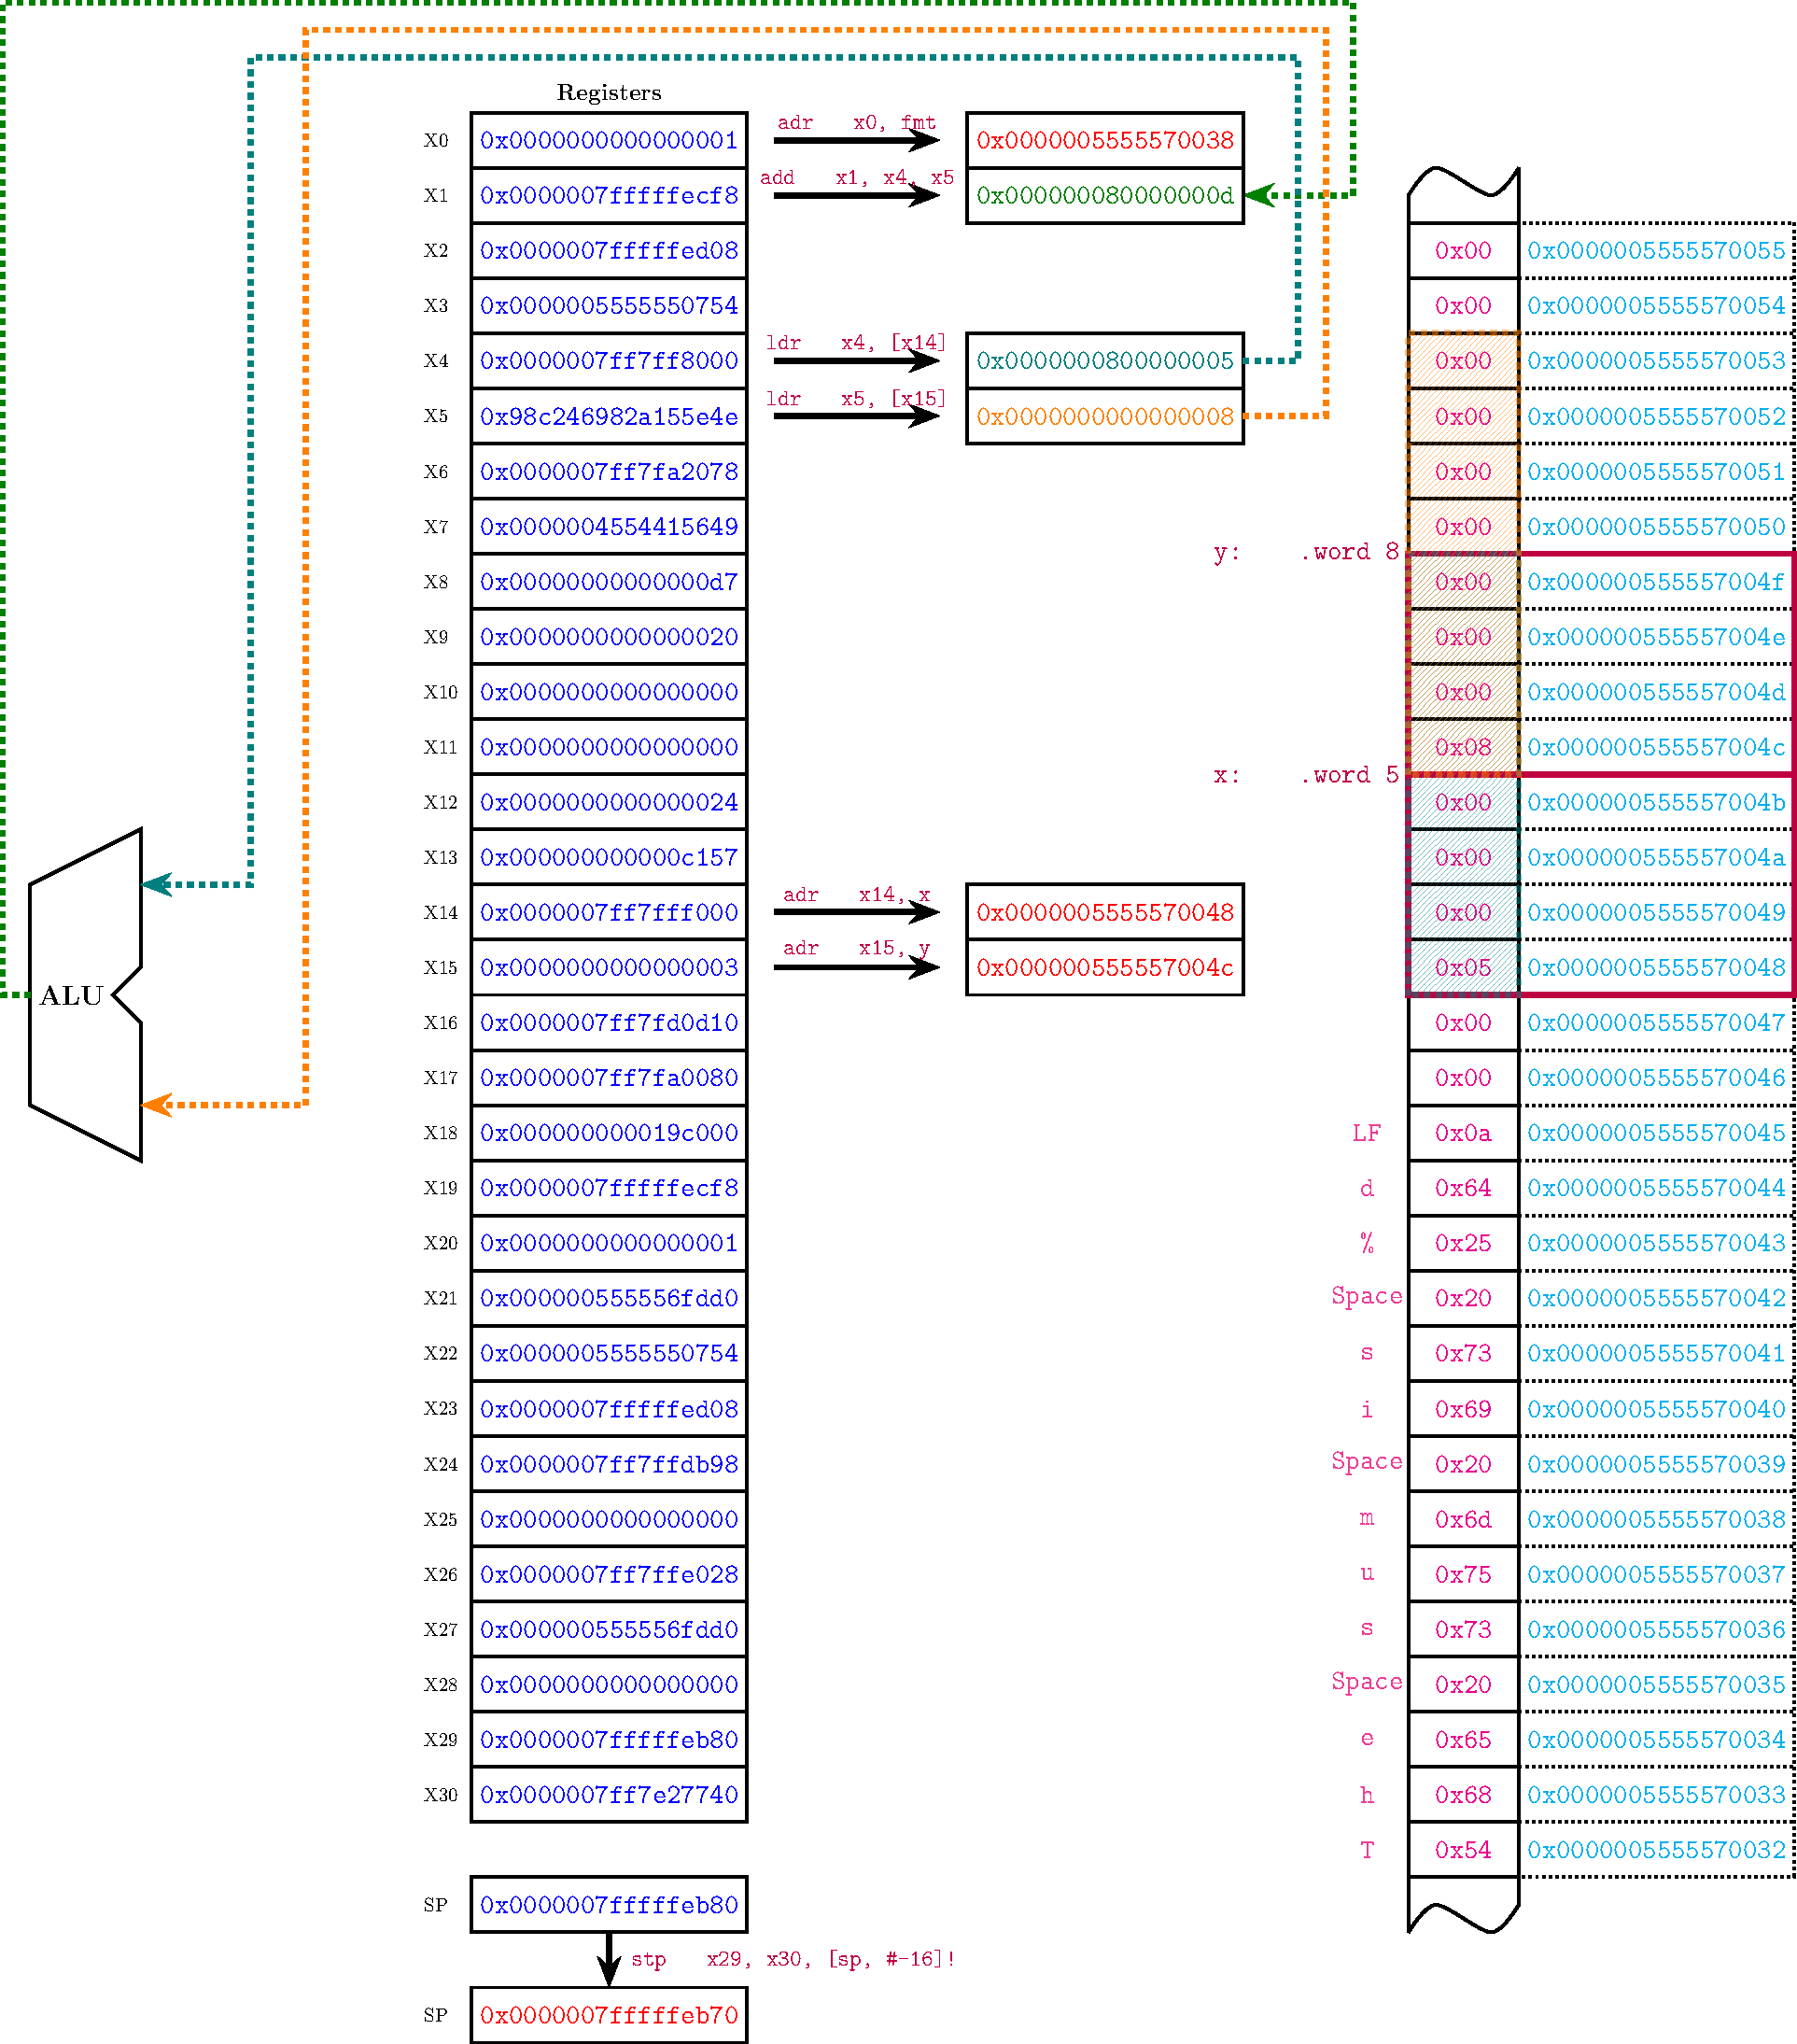
\includegraphics[width=1.5\textwidth]{architectures/sum.pdf}
\end{figure}

\newpage
\subsection{Shift Operations}
\subsection{Multiply Operations with Overflow}
\subsection{Multiply Operations with 64-bit results}
\subsection{Multiply Operations with 128-bit results}
\subsection{Division Operations}
\subsection{Comparison Operations}
\subsection{Conditional Operations}


\newpage

%----------------------------------------------------------------------------------------
%	SECTION 5 Structured Programming
%----------------------------------------------------------------------------------------
\section{Structured Programming}

\newpage



%----------------------------------------------------------------------------------------
%	SECTIONS
%----------------------------------------------------------------------------------------
\newpage
%\iffalse
\section{Section Title} % Top level section

Lorem ipsum dolor sit amet, consectetur adipiscing elit. Aliquam auctor mi risus, quis tempor libero hendrerit at. Duis hendrerit placerat quam et semper. Nam ultricies metus vehicula arcu viverra, vel ullamcorper justo elementum. Pellentesque vel mi ac lectus cursus posuere et nec ex. Fusce quis mauris egestas lacus commodo venenatis. Ut at arcu lectus. Donec et urna nunc. Morbi eu nisl cursus sapien eleifend tincidunt quis quis est. Donec ut orci ex. Praesent ligula enim, ullamcorper non lorem a, ultrices volutpat dolor. Nullam at imperdiet urna. Pellentesque nec velit eget est pretium.\sidenote{This is a sidenote. This template features a large margin specifically so you can put notes, figures, tables and other things into it as additional material to the main content in the text block.}

Donec in elit ac ante vestibulum rhoncus. Pellentesque ligula tortor, aliquet malesuada nulla tristique vitae. Aliquam mi sem, varius eu pellentesque et, tristique nec quam. Vestibulum pellentesque in dui et venenatis. Sed malesuada elit pellentesque sapien aliquet porta. In at facilisis diam. Duis id ante tellus.\sidenote[][2cm]{This sidenote has been pushed down the page manually with an optional parameter, otherwise it would be right under the one above.} % This first optional argument to a sidenote is the symbol to use (leave this empty for automatic numbering) and the second is the vertical offset (positive is down, negative is up)

\subsection{Subsection Title} % Second level section

In diam libero, vulputate quis accumsan non, auctor in ipsum. Praesent cursus velit eget lacus sodales porta. Proin quis risus ut velit euismod scelerisque ut sed neque. Cras sagittis, dolor ac ullamcorper auctor, tortor dui facilisis diam, at sagittis nisi ipsum a neque. Nullam vel mattis nisi. Ut interdum ut diam at ornare. Nulla ultrices elit justo, vitae tristique massa vulputate sit amet.

\nonumsidenote{This sidenote isn't numbered in the text or margin. This is useful for notes that apply anywhere on the page instead of one particular place.}Vestibulum erat felis, cursus vitae convallis ac, commodo eu nisi. Nulla facilisi. Mauris dignissim nisi felis, a mollis ex accumsan vel. Suspendisse bibendum vitae nibh in suscipit. Vestibulum et finibus eros. Nulla facilisi. Cras luctus aliquam finibus. In nec justo nec orci malesuada faucibus.

\subsubsection{Subsubsection Title} % Third level section

\begin{fullwidth} % Use the whole page width
	\textit{This is an example of a full width paragraph\ldots} Curabitur id placerat orci. Vivamus pulvinar augue ac feugiat blandit. Donec in ultricies mi. Nam eu lacus ac augue aliquet consectetur. Praesent dui risus, sollicitudin nec felis ut, posuere ultricies dolor. Sed massa nulla, dignissim eget sem sit amet, eleifend fermentum dui. Phasellus consequat sem vel turpis finibus, a aliquam risus malesuada.
\end{fullwidth}

Maecenas consectetur metus at tellus finibus condimentum. Proin arcu lectus, ultrices non tincidunt et, tincidunt ut quam. Integer luctus posuere est, non maximus ante dignissim quis. Nunc a cursus erat. Curabitur suscipit nibh in tincidunt sagittis. Nam malesuada vestibulum quam id gravida. Proin ut dapibus velit. Vestibulum eget quam quis ipsum semper convallis. Duis consectetur nibh ac diam dignissim, id condimentum enim dictum. Nam aliquet ligula eu magna pellentesque, nec sagittis leo lobortis. Aenean tincidunt dignissim egestas. Morbi efficitur risus ante, id tincidunt odio pulvinar vitae.

\paragraph{Paragraph Title} % Fourth level section

Lorem ipsum dolor sit amet, consectetur adipiscing elit. Aliquam auctor mi risus, quis tempor libero hendrerit at. Duis hendrerit placerat quam et semper. Nam ultricies metus vehicula arcu viverra, vel ullamcorper justo elementum. Pellentesque vel mi ac lectus cursus posuere et nec ex.

The section titles below show how multi-line section titles look at the 3 top levels.

\section[Short version of long section title]{Fusce eleifend porttitor arcu, id accumsan elit pharetra eget} % Use the optional parameter to the \section command to specify a shorter version of the title for the table of contents

Lorem ipsum dolor sit amet, consectetur adipiscing elit. \nonumsidenote[-2cm]{Section, subsection and subsubsection titles can span multiple lines, as shown here. Make sure to put a shorter version of these long titles in the optional parameter to the section commands so the title output to the table of contents is the short version.}

\subsection[Short version of long subsection title]{Phasellus sit amet enim efficitur, aliquam nulla id, lacinia mauris viverra libero ac magna}

Lorem ipsum dolor sit amet, consectetur adipiscing elit.

\subsubsection{In mi mauris, finibus non faucibus non, imperdiet nec leo. In erat arcu, tincidunt nec aliquam et, volutpat eget}

Lorem ipsum dolor sit amet, consectetur adipiscing elit.

%----------------------------------------------------------------------------------------
%	FONTS
%----------------------------------------------------------------------------------------

\section{Font Examples}

\subsection{Font Sizes}

{\tiny \textbackslash tiny} {\scriptsize \textbackslash scriptsize} {\footnotesize \textbackslash footnotesize} {\small \textbackslash small}\\
{\normalsize \textbackslash normalsize}\nonumsidenote[-1cm]{The default font size for the document is 12pt, represented by \textbackslash normalsize. The standard LaTeX font size commands modify this to be smaller or larger as needed.}\\
{\large \textbackslash large} {\Large \textbackslash Large} {\LARGE \textbackslash LARGE} {\huge \textbackslash huge} {\Huge \textbackslash Huge}

\subsection{Font Families}

\textsf{IBM Plex Sans Text}\nonumsidenote{The sans family is the default, as is standard in the business world. Use the serif family to accentuate text, such as for quotations. The mono family is best used where it's important that all characters are the same width, such as for numbers in a table or for code.}

\textrm{IBM Plex Serif Text}

\texttt{IBM Plex Mono Text}

\subsection{Font Weights}

\textel{ExtraLight} \textl{Light} Normal \textsb{SemiBold} \textbf{Bold}

\subsection{Condensed Fonts}

Plex Sans Normal\nonumsidenote{Condensed fonts can be useful if horizontal space is at a premium. You might want to use the condensed font in a wide table.}

{\plexsanscondensed Plex Sans Condensed}

%----------------------------------------------------------------------------------------
%	QUOTATIONS
%----------------------------------------------------------------------------------------

\section{Quotations}

Proin mollis urna posuere fringilla. Curabitur finibus, neque vitae vestibulum vestibulum, dolor sapien tincidunt augue, vel porta mauris metus nec mauris. Integer erat magna, porta id erat sed, lacinia volutpat erat. Nulla fermentum tellus arcu, eu iaculis ipsum malesuada aliquam. Duis et lacus maximus, consectetur metus et, eleifend arcu. Vestibulum condimentum diam vitae diam tincidunt viverra.\sidenotequote[-1cm]{\textbf{\LARGE ``}Lorem ipsum dolor sit amet, consectetur adipiscing elit. Praesent porttitor arcu luctus, imperdiet urna iaculis, mattis eros. Pellentesque iaculis odio vel nisl ullamcorper, nec faucibus ipsum molestie.\textbf{''}\\[4pt]\hfill--- John Smith, 1972} % Example margin quotation using the \sidenotequote custom command

\begin{quote}
	\textbf{\LARGE ``}Lorem ipsum dolor sit amet, consectetur adipiscing elit. Praesent porttitor arcu luctus, imperdiet urna iaculis, mattis eros. Pellentesque iaculis odio vel nisl ullamcorper, nec faucibus ipsum molestie. Sed dictum nisl non aliquet porttitor. Etiam vulputate arcu dignissim, finibus sem et, viverra nisl. Aenean luctus congue massa, ut laoreet metus ornare in.\textbf{''}
	
	\hfill--- John Smith, 1972
\end{quote}

Suspendisse tempus odio sit amet volutpat suscipit. Pellentesque ornare libero lacus, non fringilla dolor placerat in. Ut maximus ullamcorper lectus, a pharetra mi sagittis aliquet. Scelerisque augue sed mi fringilla, vel dapibus ligula finibus. Sed ornare velit sem, ac venenatis velit dignissim. Vestibulum ultrices mi at tincidunt condimentum.

%----------------------------------------------------------------------------------------
%	TABLES
%----------------------------------------------------------------------------------------

\section{Table Examples}

This statement automatically references the table below using its label: Table \ref{tab:example}.

%------------------------------------------------

\begin{margintable} % Use the margintable environment for tables to be output to the margin
	\footnotesize % Reduce the font size in the table as space is at a premium
	\caption{Margin table caption.}
	\begin{tabular}{L{0.22\linewidth} C{0.22\linewidth} R{0.25\linewidth}}
		\toprule
		\textbf{Year} & \textbf{Qtr.} & \textbf{Perf.}\\
		\midrule
		20XX & Q1 & 0.5\%\\
		20XX & Q2 & 26.5\%\\
		20XX & Q1 & 35.4\%\\
		20XX & Q4 & 41.3\%\\
		\bottomrule
	\end{tabular}
\end{margintable}

%------------------------------------------------

\begin{table}[H] % [H] forces the table to be output where it is defined in the code (it suppresses floating)
	\caption{Text block table caption.}
	\begin{tabular}{L{0.35\linewidth} L{0.38\linewidth} L{0.16\linewidth}}
		\toprule
		\textbf{Prospect} & \textbf{Industry} & \textbf{Revenue} \\
		\midrule
		Gerlach Inc & Business Development & \$3M\\
		Doyle and Sons & Law & \$1M\\
		Heathcote Group & Consulting & \$12M\\
		Goyette Inc & Advertising & \$5M\\
		Holzdeppe GmbH & Manufacturing & \$23M\\
		Bienias AG & Accounting & \$2.5M\\
		\bottomrule
	\end{tabular}
	\label{tab:example}
\end{table}

%------------------------------------------------

\begin{table*} % Use the table* environment for full width tables
	\caption{Full width table caption.}
	\begin{tabular}{C{0.03\linewidth} L{0.25\linewidth} L{0.27\linewidth} L{0.16\linewidth} L{0.16\linewidth}}
		\toprule
		\textit{\#} & \textbf{Prospect} & \textbf{Industry} & \textbf{Revenue} & \textbf{Employees} \\
		\midrule
		\textit{1} & Gerlach Inc & Business Development & \$3M & 65\\
		\textit{2} & Doyle and Sons & Law & \$1M & 15\\
		\textit{3} & Heathcote Group & Consulting & \$12M & 250\\
		\textit{4} & Goyette Inc & Advertising & \$5M & 100\\
		\textit{5} & Holzdeppe GmbH & Manufacturing & \$23M & 75\\
		\textit{6} & Bienias AG & Accounting & \$2.5M & 40\\
		\bottomrule
	\end{tabular}
\end{table*}

%----------------------------------------------------------------------------------------
%	FIGURES
%----------------------------------------------------------------------------------------

\section{Figure Examples}

This statement automatically references the figure below using its label: Figure \ref{fig:example}.

%------------------------------------------------

\begin{marginfigure} % Use the marginfigure environment for figures to be output to the margin
	
\includegraphics[width=\linewidth]{placeholder.jpg}
	\caption{Margin figure caption.}
\end{marginfigure}

%------------------------------------------------

\begin{figure}[H] % [H] forces the figure to be output where it is defined in the code (it suppresses floating)
	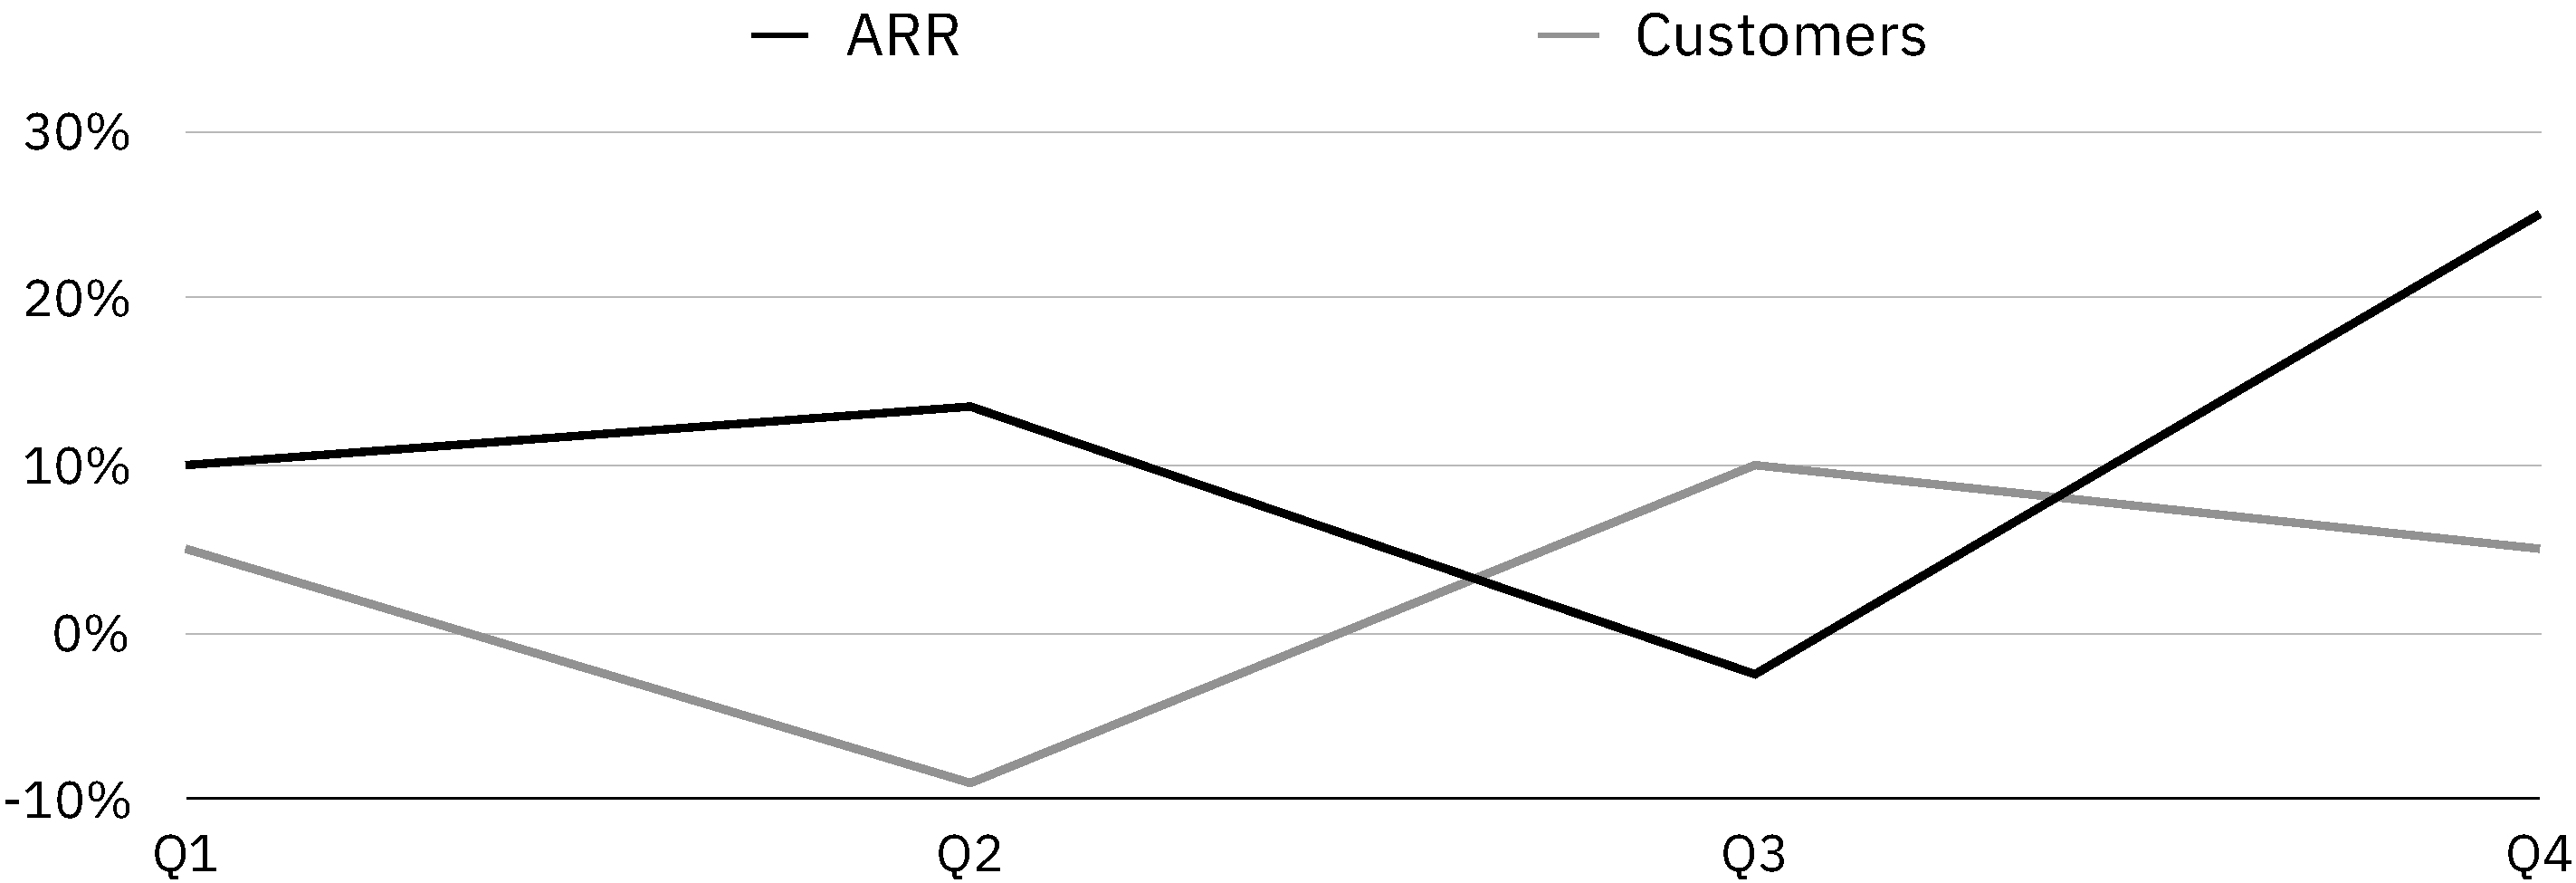
\includegraphics[width=\linewidth]{ARR.pdf}
	\caption{Text block figure caption.}
	\label{fig:example} % Label for referencing this figure in the text automatically
\end{figure}

%------------------------------------------------

\begin{figure*} % Use the figure* environment for full width figures
	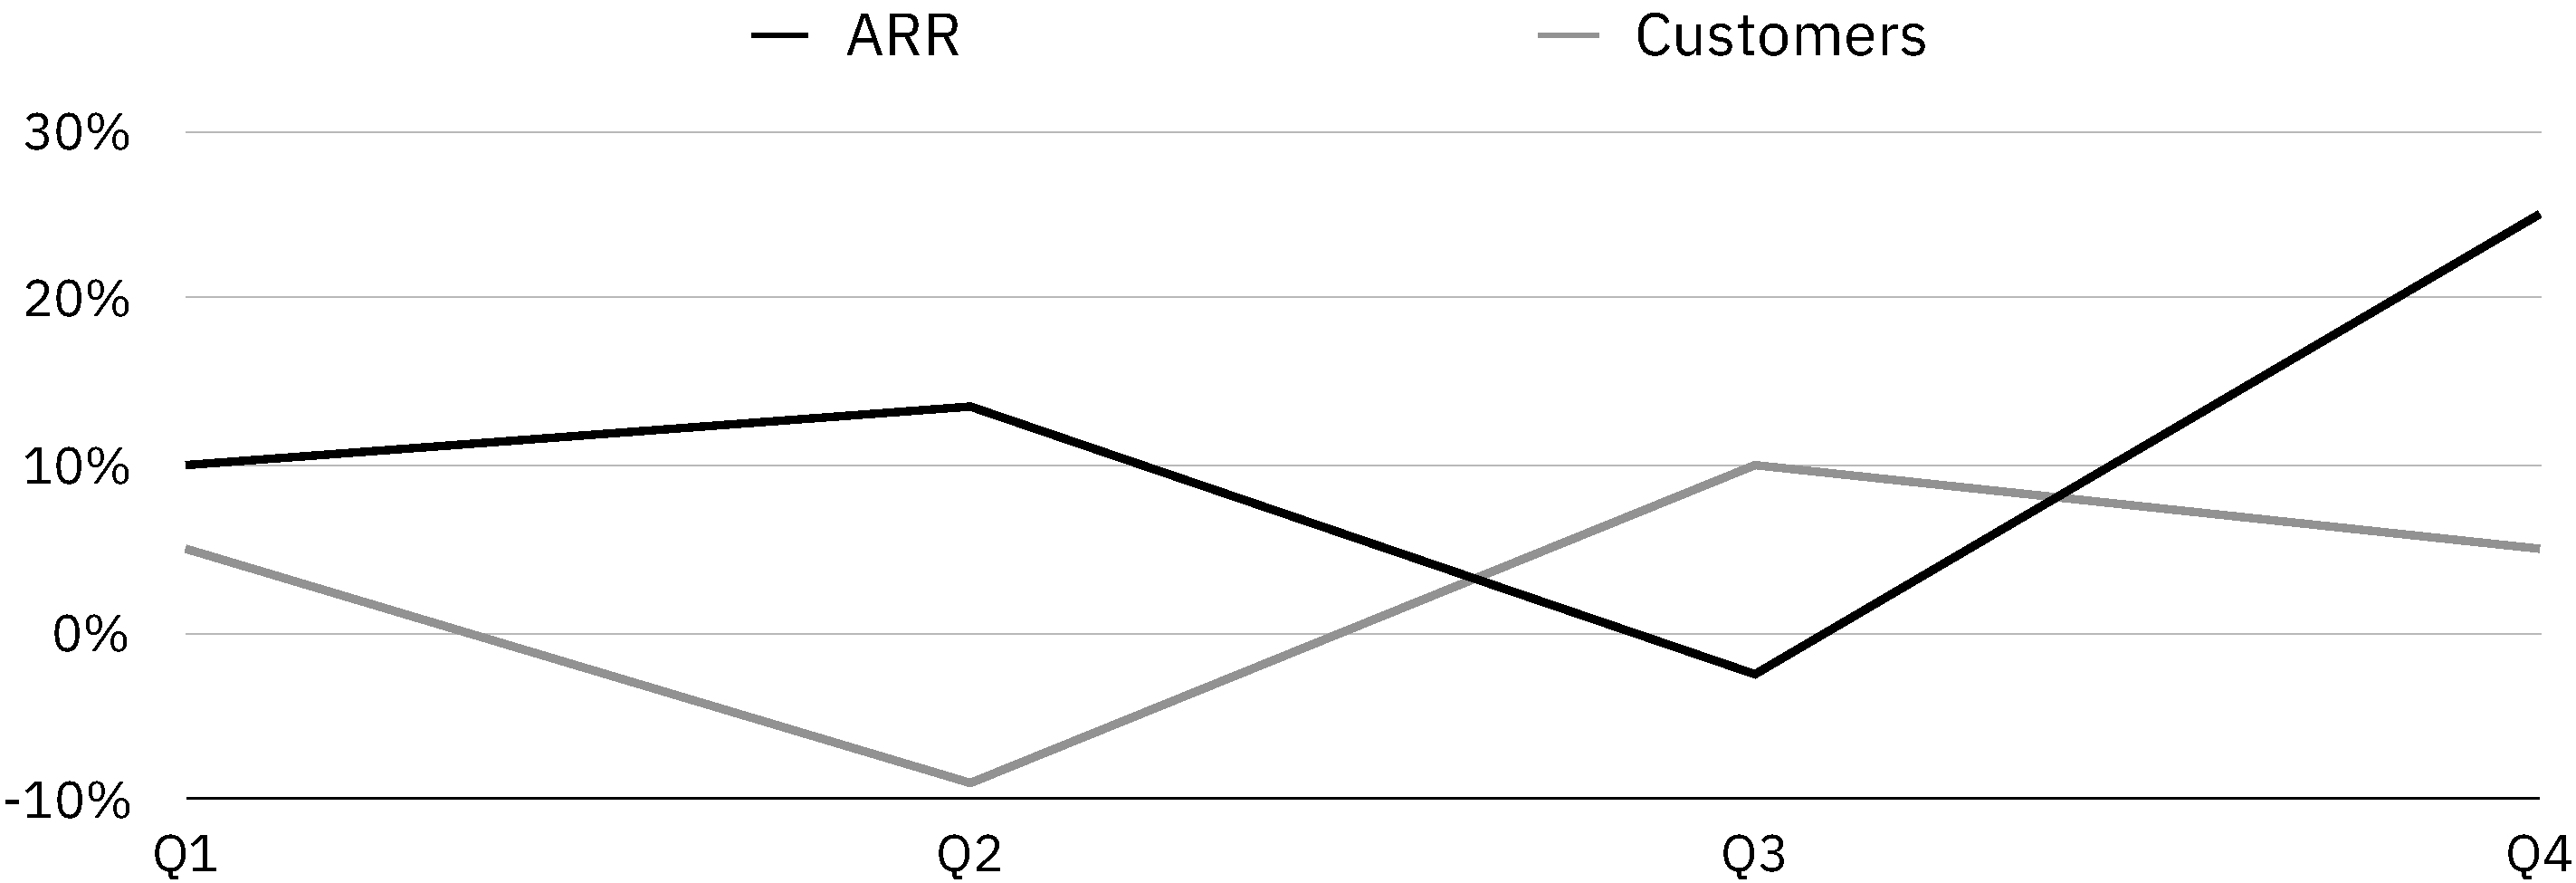
\includegraphics[width=\linewidth]{ARR.pdf}
	\caption{Full width figure caption.}
\end{figure*}

%----------------------------------------------------------------------------------------
%	LISTS
%----------------------------------------------------------------------------------------

\section{List Examples}

\subsection{Bullet Point List}

\nonumsidenote{Bullet point lists can also be created in the margin. For these, we can remove the usual left margin to increase the available horizontal space:\\\medskip \begin{itemize}[leftmargin=*]\item Bullet item one. \item Bullet item two. \item Bullet item three.\end{itemize}}Lorem ipsum dolor sit amet, consectetur adipiscing elit. Praesent porttitor arcu luctus, imperdiet urna iaculis, mattis eros. Pellentesque iaculis odio vel nisl ullamcorper, nec faucibus ipsum molestie. Sed dictum nisl non aliquet porttitor.

\begin{itemize}
	\item First bullet point item
	\begin{itemize}
		\item First indented bullet point item
		\item Second indented bullet point item
		\begin{itemize}
			\item First second-level indented bullet point item
			\item Second second-level indented bullet point item
		\end{itemize}
		\item Third indented bullet point item
	\end{itemize}
	\item Second bullet point item
	\item Third bullet point item
\end{itemize}

Etiam vulputate arcu dignissim, finibus sem et, viverra nisl. Aenean luctus congue massa, ut laoreet metus ornare in. Nunc fermentum nisi imperdiet lectus tincidunt vestibulum at ac elit. Nulla mattis nisl eu malesuada suscipit.

%------------------------------------------------

\subsection{Numbered List}

\nonumsidenote[-2.5cm]{Numbered lists can also be created in the margin. For these, we can remove the usual left margin to increase the available horizontal space:\\\medskip \begin{enumerate}[leftmargin=*]\item Numbered item one. \item Numbered item two. \item Numbered item three.\end{enumerate}}Lorem ipsum dolor sit amet, consectetur adipiscing elit. Praesent porttitor arcu luctus, imperdiet urna iaculis, mattis eros. Pellentesque iaculis odio vel nisl ullamcorper, nec faucibus ipsum molestie. Sed dictum nisl non aliquet porttitor.

\begin{enumerate}
	\item First numbered item
	\begin{enumerate}
		\item First indented numbered item
		\item Second indented numbered item
		\begin{enumerate}
			\item First second-level indented numbered item
			\item Second second-level indented numbered item
		\end{enumerate}
		\item Third indented numbered item
	\end{enumerate}
	\item Second numbered item
	\item Third numbered item
\end{enumerate}

Etiam vulputate arcu dignissim, finibus sem et, viverra nisl. Aenean luctus congue massa, ut laoreet metus ornare in. Nunc fermentum nisi imperdiet lectus tincidunt vestibulum at ac elit. Nulla mattis nisl eu malesuada suscipit.

%------------------------------------------------

\subsection{Description List}

\nonumsidenote{Description lists can also be created in the margin:\\\medskip \begin{description}\item[A1] Description item one. \item[B1] Description item two. \item[C1] Description item three.\end{description}}Lorem ipsum dolor sit amet, consectetur adipiscing elit. Praesent porttitor arcu luctus, imperdiet urna iaculis, mattis eros. Pellentesque iaculis odio vel nisl ullamcorper, nec faucibus ipsum molestie. Sed dictum nisl non aliquet porttitor.

\begin{description}
	\item[Item One] Lorem ipsum dolor sit amet, consectetur adipiscing elit. Praesent porttitor arcu luctus, imperdiet urna iaculis, mattis eros. Pellentesque iaculis odio vel nisl ullamcorper, nec faucibus ipsum molestie.
	\item[Item Two] Sed dictum nisl non aliquet porttitor.
	\begin{description}
		\item[Subitem] Maecenas consectetur metus at tellus finibus condimentum. Proin arcu lectus, ultrices non tincidunt et, tincidunt ut quam. Integer luctus posuere est, non maximus ante dignissim quis.
		\begin{description}
			\item[Subsubitem] Maecenas consectetur metus at tellus finibus condimentum. Proin arcu lectus, ultrices non tincidunt et, tincidunt ut quam. Integer luctus posuere est, non maximus ante dignissim quis.
	\end{description}
	\end{description}
	\item[Item Three] Etiam vulputate arcu dignissim, finibus sem et, viverra nisl. Aenean luctus congue massa, ut laoreet metus ornare in. Nunc fermentum nisi imperdiet lectus tincidunt vestibulum at ac elit. Nulla mattis nisl eu malesuada suscipit.
\end{description}

Etiam vulputate arcu dignissim, finibus sem et, viverra nisl. Aenean luctus congue massa, ut laoreet metus ornare in.

%----------------------------------------------------------------------------------------
%	REFERENCING CITATIONS
%----------------------------------------------------------------------------------------

\section{Referencing Citations}

This statement requires citation \autocite{Smith:2024jd}.

This statement requires multiple citations \autocite{Smith:2024jd, Smith:2023qr}.

This short citation is in the margin\sidecite{Smith:2023qr}.

This long citation is in the margin\fullsidecite{Smith:2024jd}.

This statement has an in-text citation: \textcite{Smith:2024jd}.

%----------------------------------------------------------------------------------------
%	LINKS
%----------------------------------------------------------------------------------------

\section{Link Examples}

This is a URL link: \href{https://www.duckduckgo.com}{DuckDuckGo}.\nonumsidenote{Links can be clicked in the PDF to navigate to the linked website or email address.}

This is a email link: \href{mailto:example@example.com}{example@example.com}.

This is a monospaced URL link: \url{https://duckduckgo.com}.

%----------------------------------------------------------------------------------------
%	EQUATIONS
%----------------------------------------------------------------------------------------

\section{Equation}

\begin{equation}
	\cos^3 \theta =\frac{1}{4}\cos\theta+\frac{3}{4}\cos 3\theta
	\label{eq:example}
\end{equation}

This statement automatically references the equation above using its label: Equation \ref{eq:example}.

%----------------------------------------------------------------------------------------
%	INTERNATIONAL SUPPORT
%----------------------------------------------------------------------------------------

\section{International Support}

àáâäãåèéêëìíîïòóôöõøùúûüÿýñçčšž\nonumsidenote{Plex is a very high quality typeface produced by IBM. It includes extensive international support and characters.}

ÀÁÂÄÃÅÈÉÊËÌÍÎÏÒÓÔÖÕØÙÚÛÜŸÝÑ

ßÇŒÆČŠŽ

%----------------------------------------------------------------------------------------
%	CODE
%----------------------------------------------------------------------------------------

\section{Displaying Code}

The block below is a code listing. It displays code in an easy to use way with line numbers for quick reference to specific parts of the code.

\begin{lstlisting}
{
	"city": [
		{
			"id": 1,
			"name": "Toronto",
			"country": "Canada",
			"population": 6200000
		},
		{
			"id": 2,
			"name": "New York",
			"country": "United States of America",
			"population": 8800000
		}
	]
}
\end{lstlisting}

%----------------------------------------------------------------------------------------
%	 REFERENCES/BIBLIOGRAPHY
%----------------------------------------------------------------------------------------

\newpage

\addcontentsline{toc}{section}{Reference List} % Add the bibliography to the table of contents

\begin{twothirdswidth} % Content in this environment to be at two-thirds of the whole page width
	\printbibliography
%	\printbibliography[title=Reference List] % Output the bibliography with a custom section title
\end{twothirdswidth}

%----------------------------------------------------------------------------------------
%	APPENDICES
%----------------------------------------------------------------------------------------

\newpage

\section*{Appendices}

\begin{appendices}

%----------------------------------------------------------------------------------------
%	SECTION 5 Structured Programming
%----------------------------------------------------------------------------------------
\section*{Big Number Addition}

\lstinputlisting[]{codes/bn_add_asm.s}

\begin{figure}[h!]\centering
	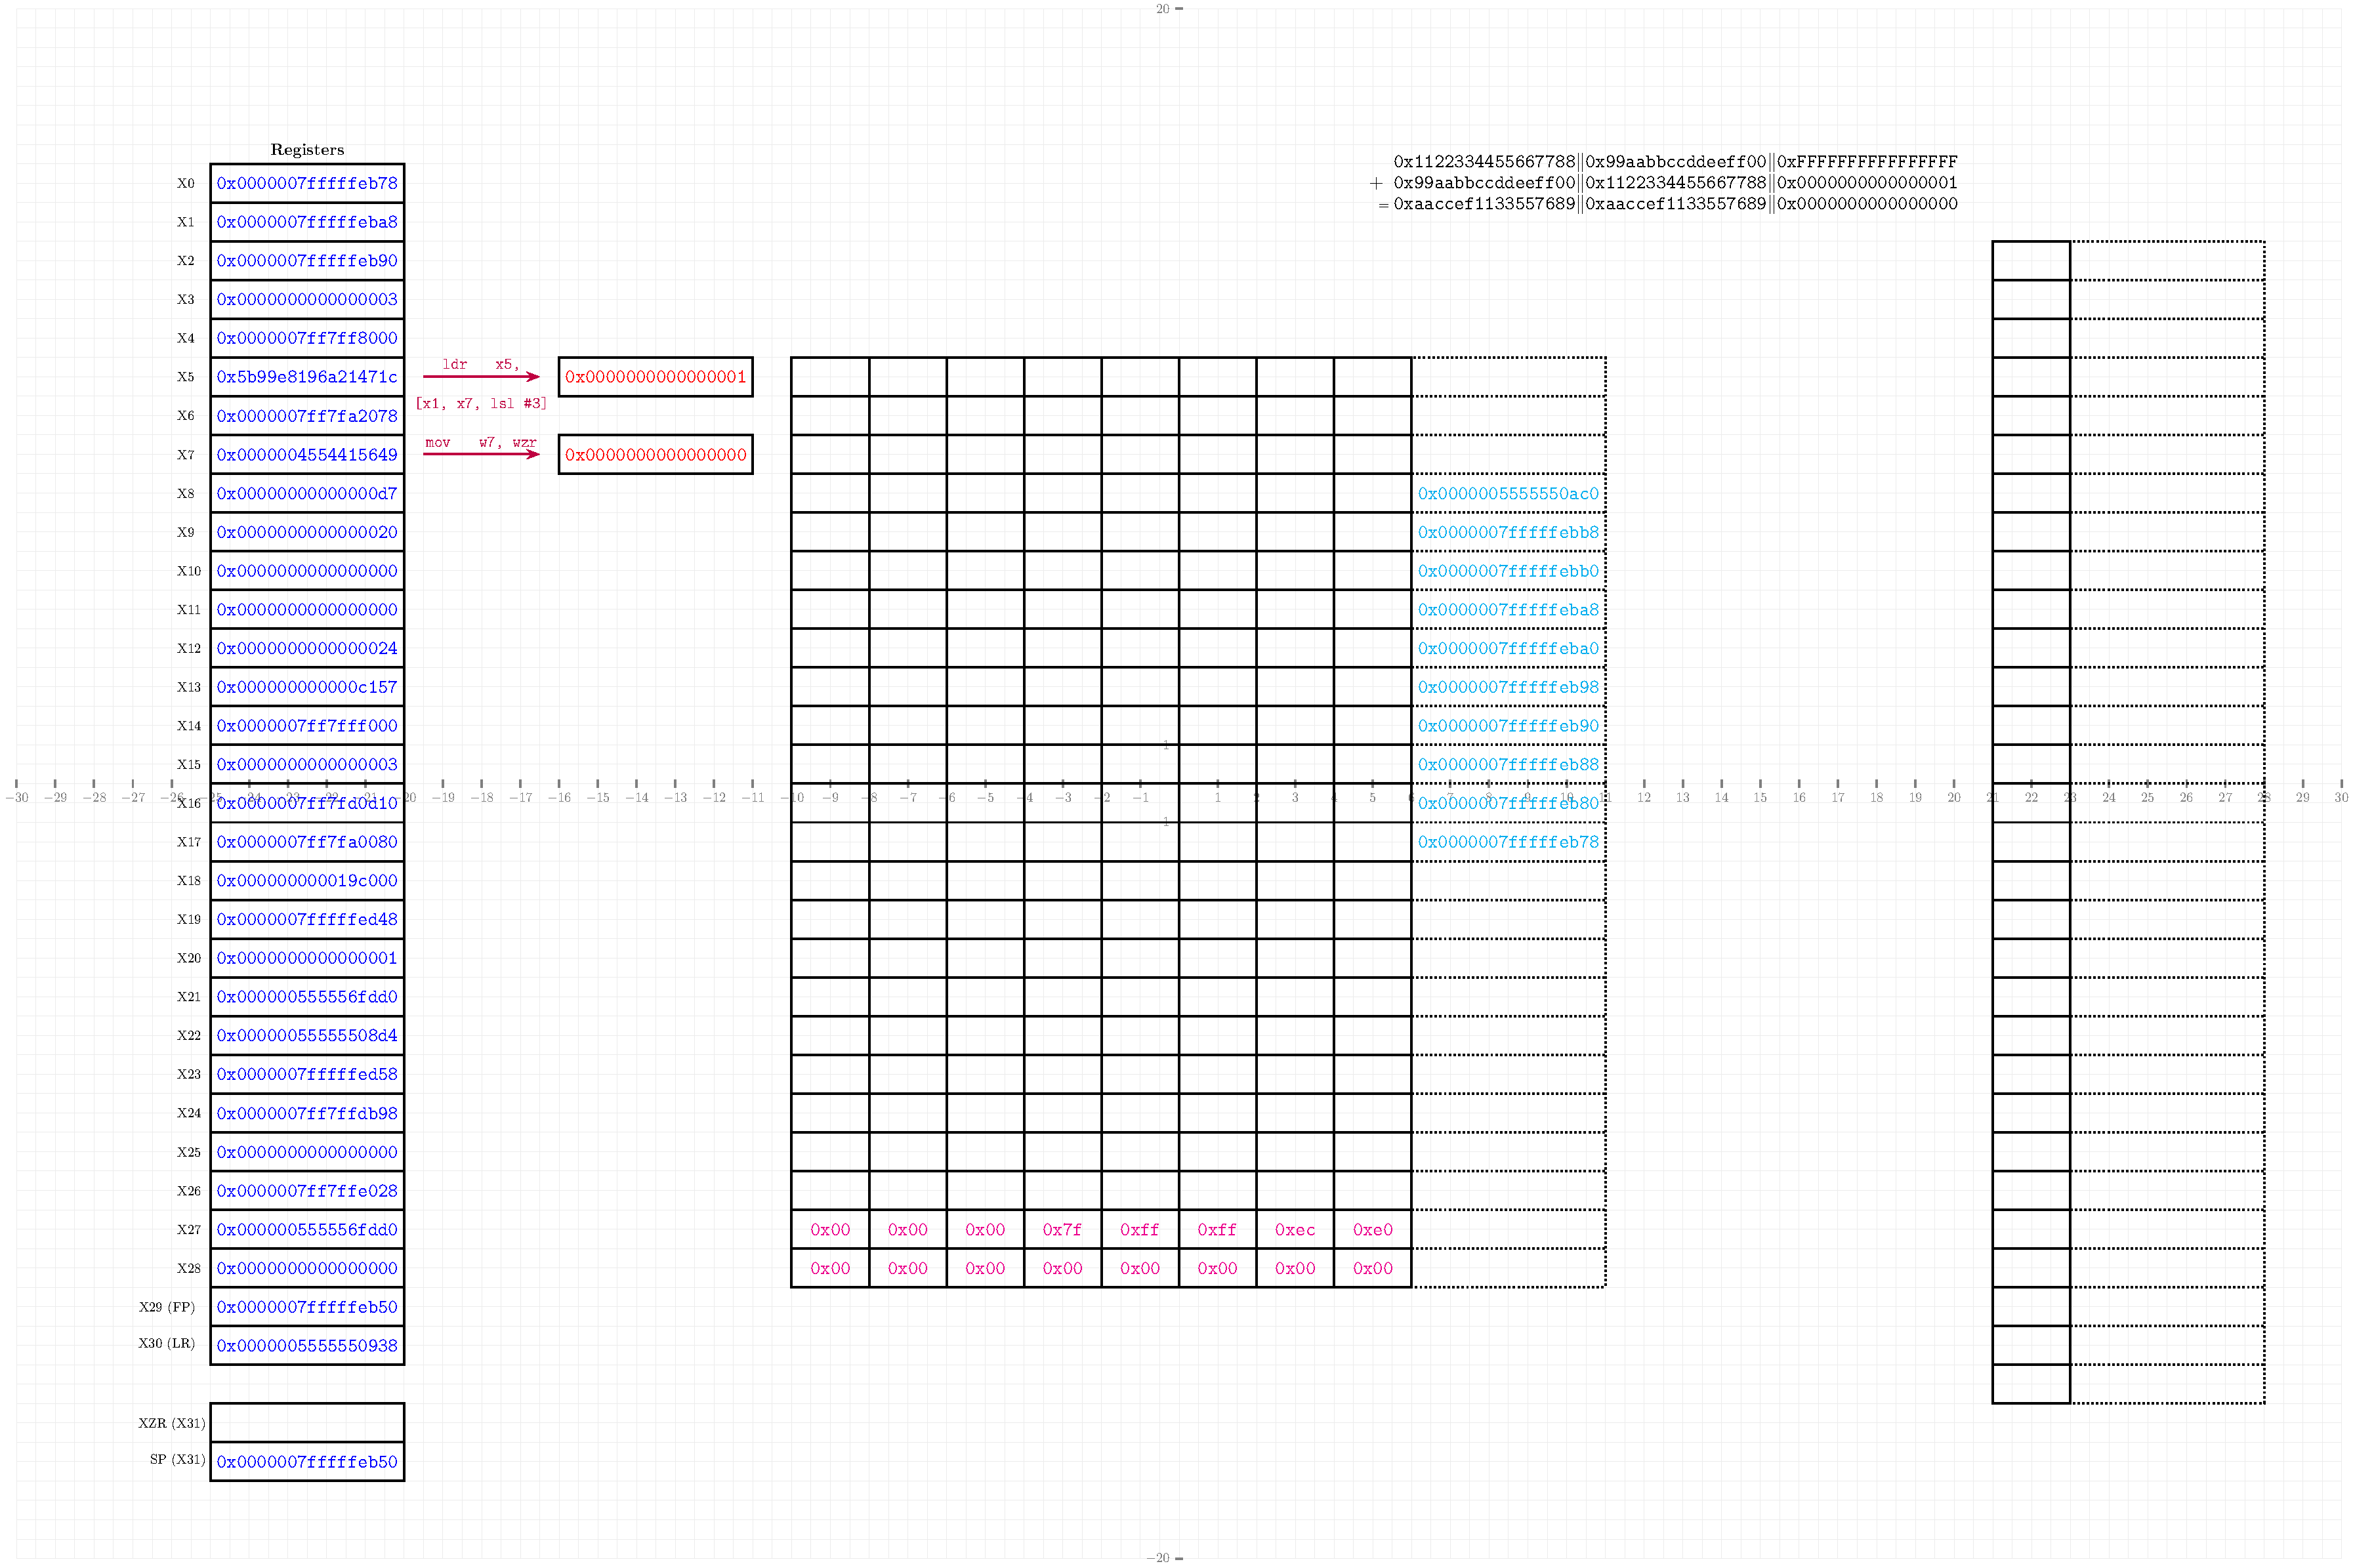
\includegraphics[width=1.5\textwidth]{architectures/bn_add.pdf}
\end{figure}
\newpage

\section{Big Nu}

Lorem ipsum dolor sit amet, consectetur adipiscing elit. Aliquam auctor mi risus, quis tempor libero hendrerit at. Duis hendrerit placerat quam et semper. Nam ultricies metus vehicula arcu viverra, vel ullamcorper justo elementum. Pellentesque vel mi ac lectus cursus posuere et nec ex. Fusce quis mauris egestas lacus commodo venenatis. Ut at arcu lectus. Donec et urna nunc. Morbi eu nisl cursus sapien eleifend tincidunt quis quis est. Donec ut orci ex. Praesent ligula enim, ullamcorper non lorem a, ultrices volutpat dolor. Nullam at imperdiet urna. Pellentesque nec velit eget euismod pretium.

\section{Appendix Section}

Lorem ipsum dolor sit amet, consectetur adipiscing elit. Aliquam auctor mi risus, quis tempor libero hendrerit at. Duis hendrerit placerat quam et semper. Nam ultricies metus vehicula arcu viverra, vel ullamcorper justo elementum. Pellentesque vel mi ac lectus cursus posuere et nec ex. Fusce quis mauris egestas lacus commodo venenatis. Ut at arcu lectus. Donec et urna nunc. Morbi eu nisl cursus sapien eleifend tincidunt quis quis est. Donec ut orci ex. Praesent ligula enim, ullamcorper non lorem a, ultrices volutpat dolor. Nullam at imperdiet urna. Pellentesque nec velit eget euismod pretium.

\section{Appendix Section}

Lorem ipsum dolor sit amet, consectetur adipiscing elit. Aliquam auctor mi risus, quis tempor libero hendrerit at. Duis hendrerit placerat quam et semper. Nam ultricies metus vehicula arcu viverra, vel ullamcorper justo elementum. Pellentesque vel mi ac lectus cursus posuere et nec ex. Fusce quis mauris egestas lacus commodo venenatis. Ut at arcu lectus. Donec et urna nunc. Morbi eu nisl cursus sapien eleifend tincidunt quis quis est. Donec ut orci ex. Praesent ligula enim, ullamcorper non lorem a, ultrices volutpat dolor. Nullam at imperdiet urna. Pellentesque nec velit eget euismod pretium.

\end{appendices}

%----------------------------------------------------------------------------------------
%\fi
\end{document}
